\subsection{Elektromagnetische Wellen auf Leitungen} % (fold)
\label{sub:elektromagnetische_wellen_auf_leitungen}

	Für die folgenden Messwerte wurden mithilfe des Frequenzgenerators immer Sinussignale mit einer Effektivspannung von $1.00$V erzeugt.
	Dies entspricht einer Peak-to-Peak-Spannung von rund $2.28$V.
	Aufgrund des verwendeten 10:1-Teilers entspricht also die zu erwartende Peak-to-Peak-Spannung des gemessenen Signales ungefähr $228$mV.

	Der Eingangs- bzw. Ausgangswiderstand des Generators beträgt immer $50\Omega$.\\

	\subsubsection{Laborkabel} % (fold)
	\label{ssub:laborkabel}
	
		Um die Komplexität von hochfrequenten Signalen zu verbildlichen, wurden als erstes Zweidrahtleitungen, welche auch als typische Laborkabel verwendet werden, vermessen. 
		Zunächst wurde eine Leitung von ca. $2$m Länge verwendet. 
		Die folgende Aufnahme \ref{versuchsaufbau_laborkabel} zeigt den genauen Aufbau:

		\begin{figure}[H]
			\center
			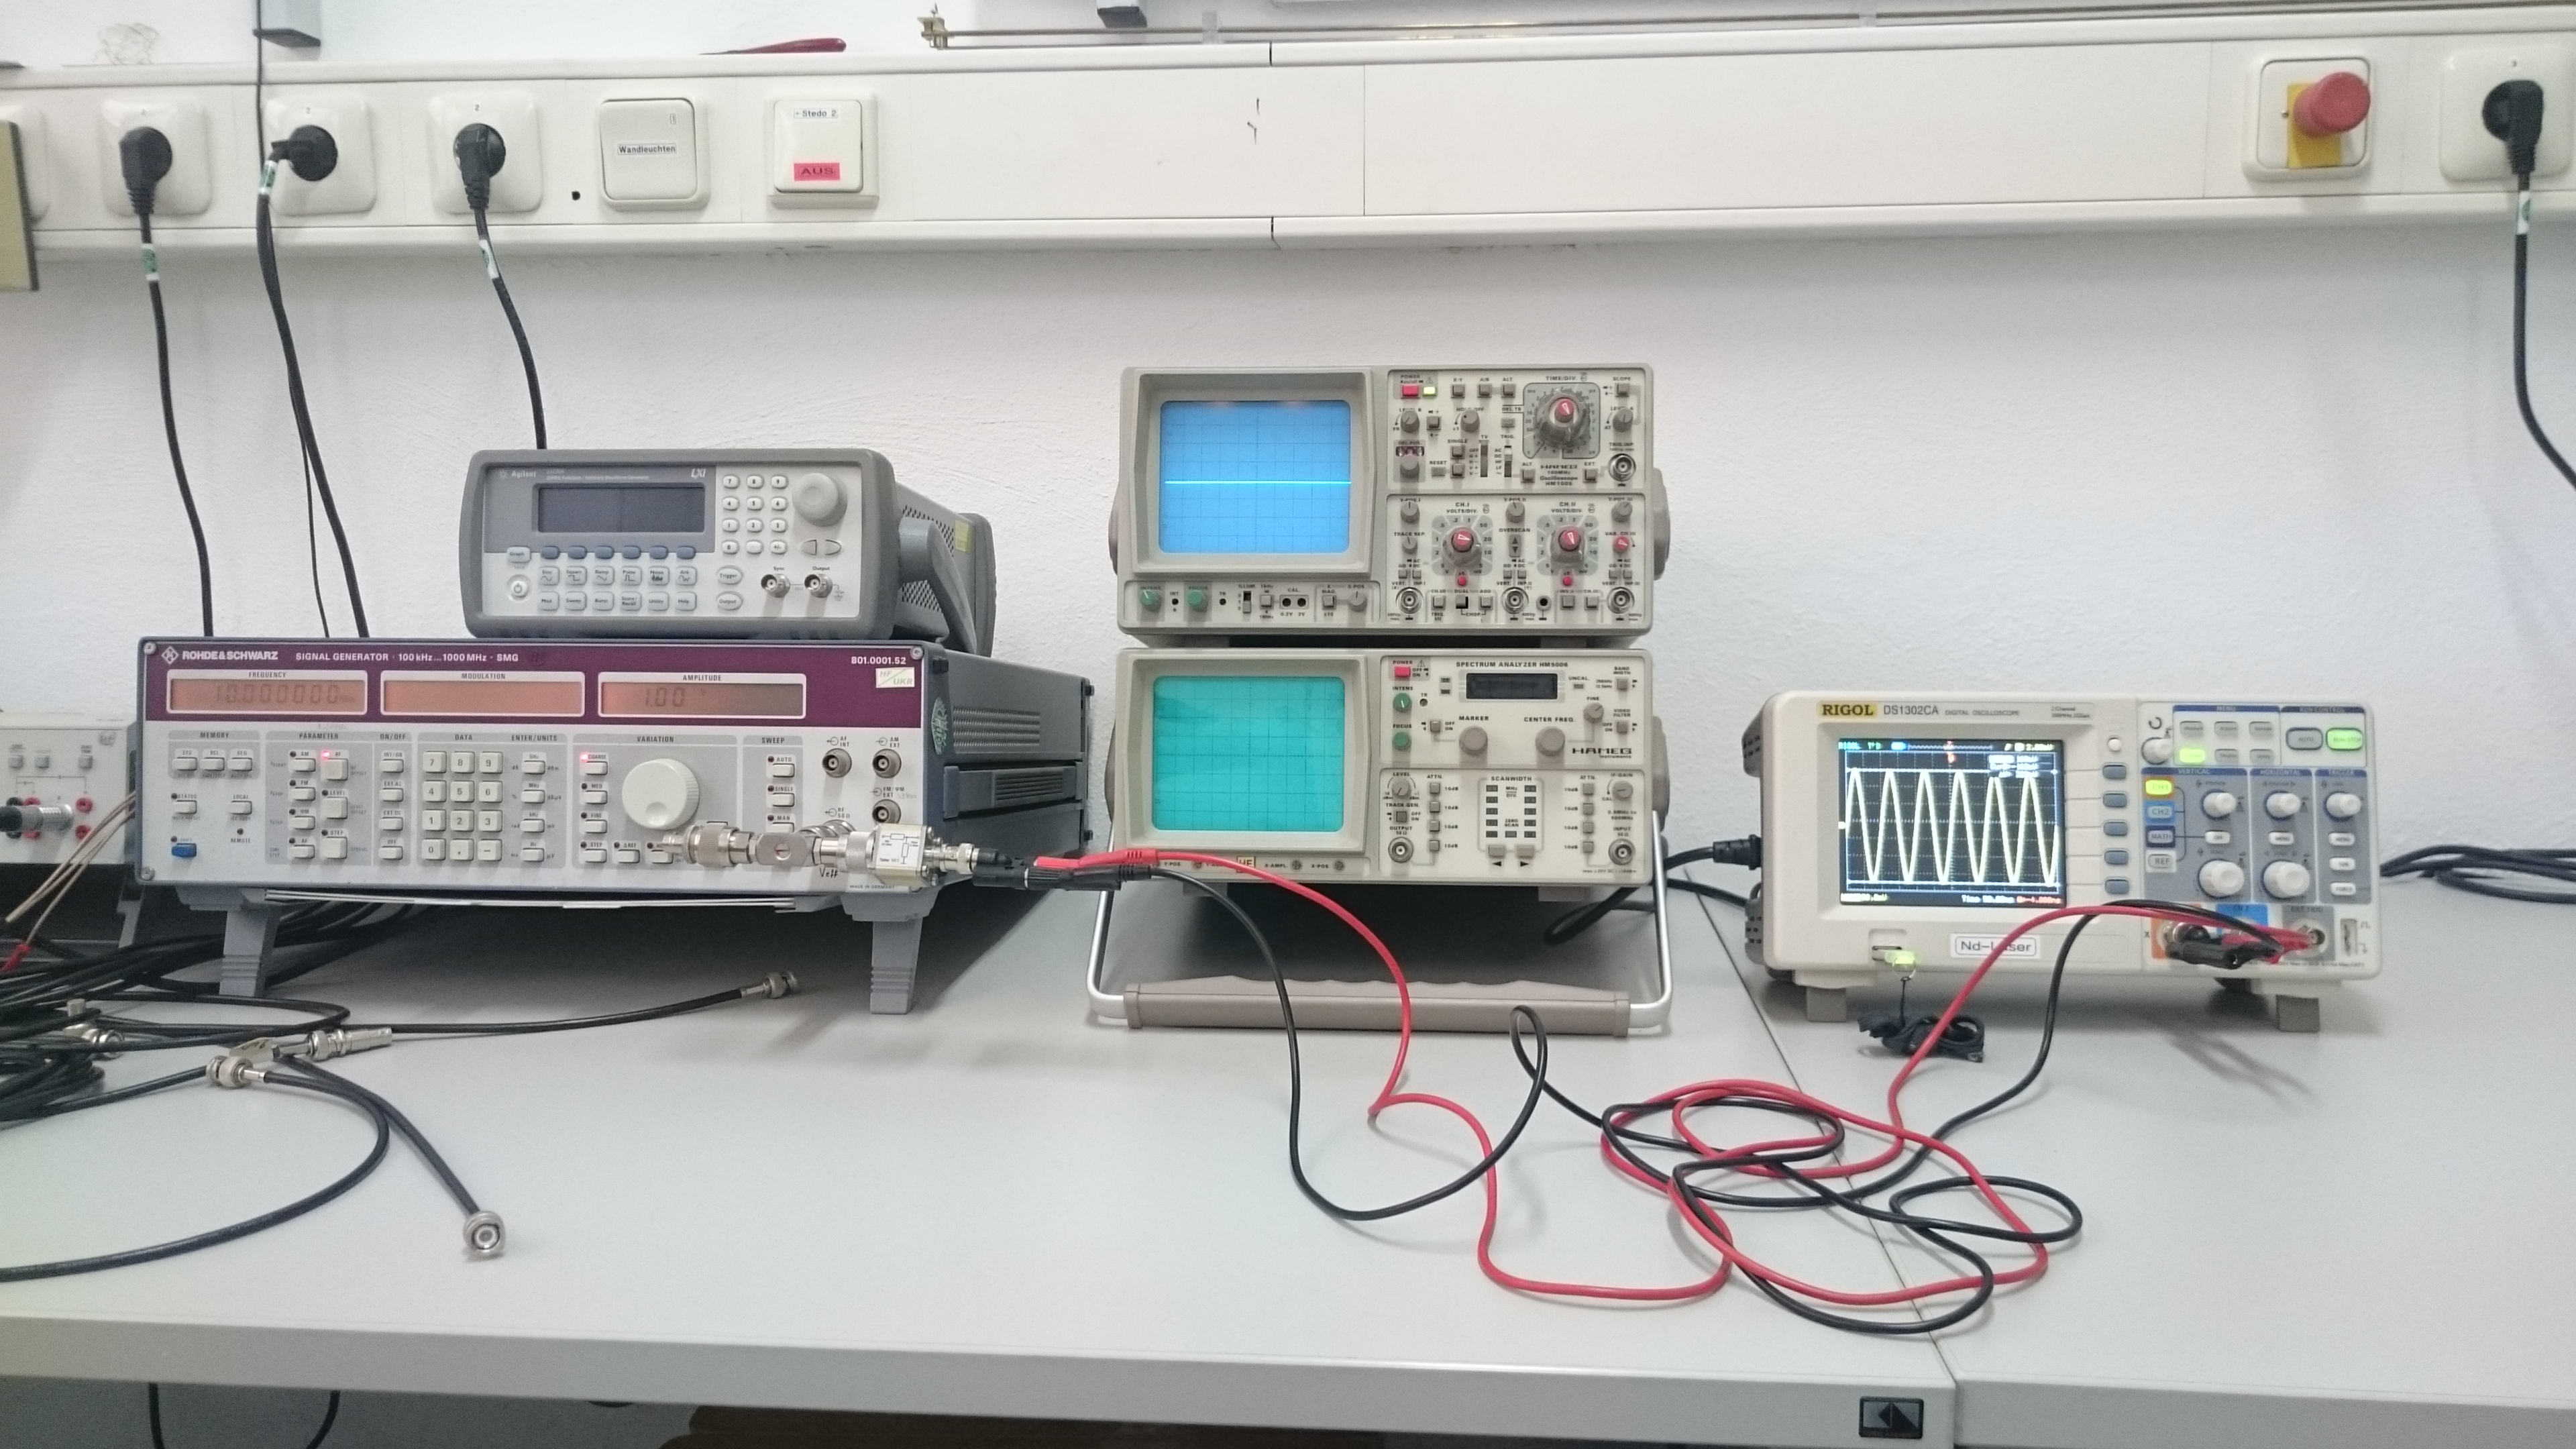
\includegraphics[scale = 0.09]{messwerte/DSC_0548.JPG}
			\caption{\centering Aufnahme des genauen Versuchsaufbaus für die verwendeten Laborkabel} %fick dich schröter!!!
			\label{versuchsaufbau_laborkabel}
		\end{figure}

		Die gemessene Übertragungsfunktion für verschiedene Eingangswiderstände am Oszilloskop ist in Abbildung \ref{diagramm_laborkabel} zu sehen.

		\begin{figure}[H]
			\center
			% GNUPLOT: LaTeX picture with Postscript
\begingroup
  \makeatletter
  \providecommand\color[2][]{%
    \GenericError{(gnuplot) \space\space\space\@spaces}{%
      Package color not loaded in conjunction with
      terminal option `colourtext'%
    }{See the gnuplot documentation for explanation.%
    }{Either use 'blacktext' in gnuplot or load the package
      color.sty in LaTeX.}%
    \renewcommand\color[2][]{}%
  }%
  \providecommand\includegraphics[2][]{%
    \GenericError{(gnuplot) \space\space\space\@spaces}{%
      Package graphicx or graphics not loaded%
    }{See the gnuplot documentation for explanation.%
    }{The gnuplot epslatex terminal needs graphicx.sty or graphics.sty.}%
    \renewcommand\includegraphics[2][]{}%
  }%
  \providecommand\rotatebox[2]{#2}%
  \@ifundefined{ifGPcolor}{%
    \newif\ifGPcolor
    \GPcolorfalse
  }{}%
  \@ifundefined{ifGPblacktext}{%
    \newif\ifGPblacktext
    \GPblacktexttrue
  }{}%
  % define a \g@addto@macro without @ in the name:
  \let\gplgaddtomacro\g@addto@macro
  % define empty templates for all commands taking text:
  \gdef\gplbacktext{}%
  \gdef\gplfronttext{}%
  \makeatother
  \ifGPblacktext
    % no textcolor at all
    \def\colorrgb#1{}%
    \def\colorgray#1{}%
  \else
    % gray or color?
    \ifGPcolor
      \def\colorrgb#1{\color[rgb]{#1}}%
      \def\colorgray#1{\color[gray]{#1}}%
      \expandafter\def\csname LTw\endcsname{\color{white}}%
      \expandafter\def\csname LTb\endcsname{\color{black}}%
      \expandafter\def\csname LTa\endcsname{\color{black}}%
      \expandafter\def\csname LT0\endcsname{\color[rgb]{1,0,0}}%
      \expandafter\def\csname LT1\endcsname{\color[rgb]{0,1,0}}%
      \expandafter\def\csname LT2\endcsname{\color[rgb]{0,0,1}}%
      \expandafter\def\csname LT3\endcsname{\color[rgb]{1,0,1}}%
      \expandafter\def\csname LT4\endcsname{\color[rgb]{0,1,1}}%
      \expandafter\def\csname LT5\endcsname{\color[rgb]{1,1,0}}%
      \expandafter\def\csname LT6\endcsname{\color[rgb]{0,0,0}}%
      \expandafter\def\csname LT7\endcsname{\color[rgb]{1,0.3,0}}%
      \expandafter\def\csname LT8\endcsname{\color[rgb]{0.5,0.5,0.5}}%
    \else
      % gray
      \def\colorrgb#1{\color{black}}%
      \def\colorgray#1{\color[gray]{#1}}%
      \expandafter\def\csname LTw\endcsname{\color{white}}%
      \expandafter\def\csname LTb\endcsname{\color{black}}%
      \expandafter\def\csname LTa\endcsname{\color{black}}%
      \expandafter\def\csname LT0\endcsname{\color{black}}%
      \expandafter\def\csname LT1\endcsname{\color{black}}%
      \expandafter\def\csname LT2\endcsname{\color{black}}%
      \expandafter\def\csname LT3\endcsname{\color{black}}%
      \expandafter\def\csname LT4\endcsname{\color{black}}%
      \expandafter\def\csname LT5\endcsname{\color{black}}%
      \expandafter\def\csname LT6\endcsname{\color{black}}%
      \expandafter\def\csname LT7\endcsname{\color{black}}%
      \expandafter\def\csname LT8\endcsname{\color{black}}%
    \fi
  \fi
  \setlength{\unitlength}{0.0500bp}%
  \begin{picture}(7370.00,3968.00)%
    \gplgaddtomacro\gplbacktext{%
      \csname LTb\endcsname%
      \put(946,704){\makebox(0,0)[r]{\strut{} 0}}%
      \put(946,1079){\makebox(0,0)[r]{\strut{} 50}}%
      \put(946,1454){\makebox(0,0)[r]{\strut{} 100}}%
      \put(946,1829){\makebox(0,0)[r]{\strut{} 150}}%
      \put(946,2204){\makebox(0,0)[r]{\strut{} 200}}%
      \put(946,2578){\makebox(0,0)[r]{\strut{} 250}}%
      \put(946,2953){\makebox(0,0)[r]{\strut{} 300}}%
      \put(946,3328){\makebox(0,0)[r]{\strut{} 350}}%
      \put(946,3703){\makebox(0,0)[r]{\strut{} 400}}%
      \put(1078,484){\makebox(0,0){\strut{} 0}}%
      \put(2061,484){\makebox(0,0){\strut{} 50}}%
      \put(3043,484){\makebox(0,0){\strut{} 100}}%
      \put(4026,484){\makebox(0,0){\strut{} 150}}%
      \put(5008,484){\makebox(0,0){\strut{} 200}}%
      \put(5991,484){\makebox(0,0){\strut{} 250}}%
      \put(6973,484){\makebox(0,0){\strut{} 300}}%
      \put(176,2203){\rotatebox{-270}{\makebox(0,0){\strut{}$U_{pp}$ \ [mV]}}}%
      \put(4025,154){\makebox(0,0){\strut{}$f$ \ [MHz]}}%
    }%
    \gplgaddtomacro\gplfronttext{%
      \csname LTb\endcsname%
      \put(5986,3530){\makebox(0,0)[r]{\strut{}Messwerte mit $R_{in} = 1$M$\Omega$}}%
      \csname LTb\endcsname%
      \put(5986,3310){\makebox(0,0)[r]{\strut{}Messwerte mit $R_{in} = 50\Omega$}}%
    }%
    \gplbacktext
    \put(0,0){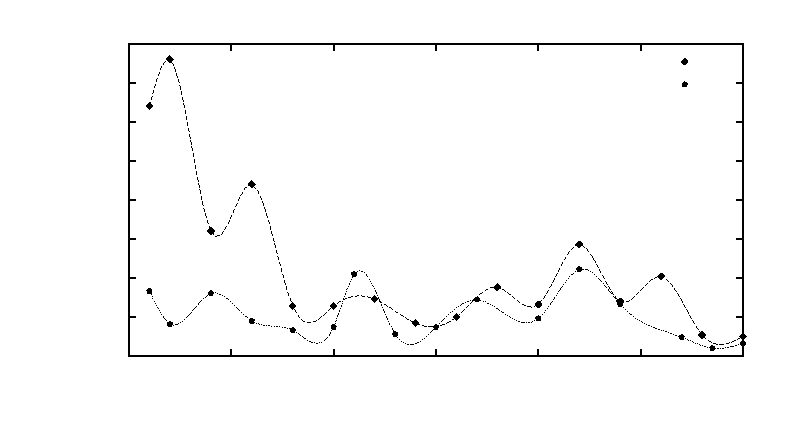
\includegraphics{laborkabel}}%
    \gplfronttext
  \end{picture}%
\endgroup

			\caption{\centering gemessene Übertragungsfunktion der Laborkabel: Peak-to-Peak-Spannung $U_{pp}$ über Frequenz $f$ bei verwendetem Eingangswiderstand $R_{in}$ am Oszilloskop} %fick dich schröter
			\label{diagramm_laborkabel}
		\end{figure}

		An dieser Stelle möchten wir noch bemerken, dass schon durch geringe Veränderungen der Lage des Kabels große Schwankungen der Peak-to-Peak-Spannung von über $50$\% beobachtet werden konnten.
		Auch sonst schwankt die Spannung je nach verwendeter Frequenz sehr stark und unregelmäßig.
		Es wird also deutlich, dass das Verhalten hochfrequenter Signale auf Leitungen anders ist als das der Niederfrequenten, da keine konstante Übertragungsfunktion gemessen werden konnte.
		Ursachen für beide Effekte liegen in der inkorrekten Anpassung des Wellenwiderstandes und des Eingangswiderstands.
		Durch Veränderung der Form des Kabels ändern sich die jeweiligen Beläge (siehe Grundlagen) und somit auch der Wellenwiderstand.
		Dieser Effekt wird verstärkt durch die nicht vorhandene Abschirmung des Kabels, da entstehende Felder des Kabels an verschiedenen Stellen wechselwirken können. \\

		Folglich ist es denkbar ungünstig typische Laborkabel für die Übertragung hochfrequenter Signale zu nutzen, da durch sie nicht quantifizierbare Effekte entstehen.

	% subsubsection laborkabel (end)

	\subsubsection{Koaxialkabel} % (fold)
	\label{ssub:koaxialkabel}
	
		Zur Verringerung des oben beschriebenen Effekts, sollen nun Koaxialkabel vermessen werden.
		Diese besitzen eine Abschirmung und einen im Wesentlichen konstanten Wellenwiderstand von $50\Omega$.
		Das zur Messung verwendete Kabel besaß eine Länge von ungefähr $1$m.
		Abbildung \ref{versuchsaufbau_koaxialkabel} zeigt eine Aufnahme des Versuchsaufbaus für die Vermessung dieses Kabels.

		\begin{figure}[H]
			\center
			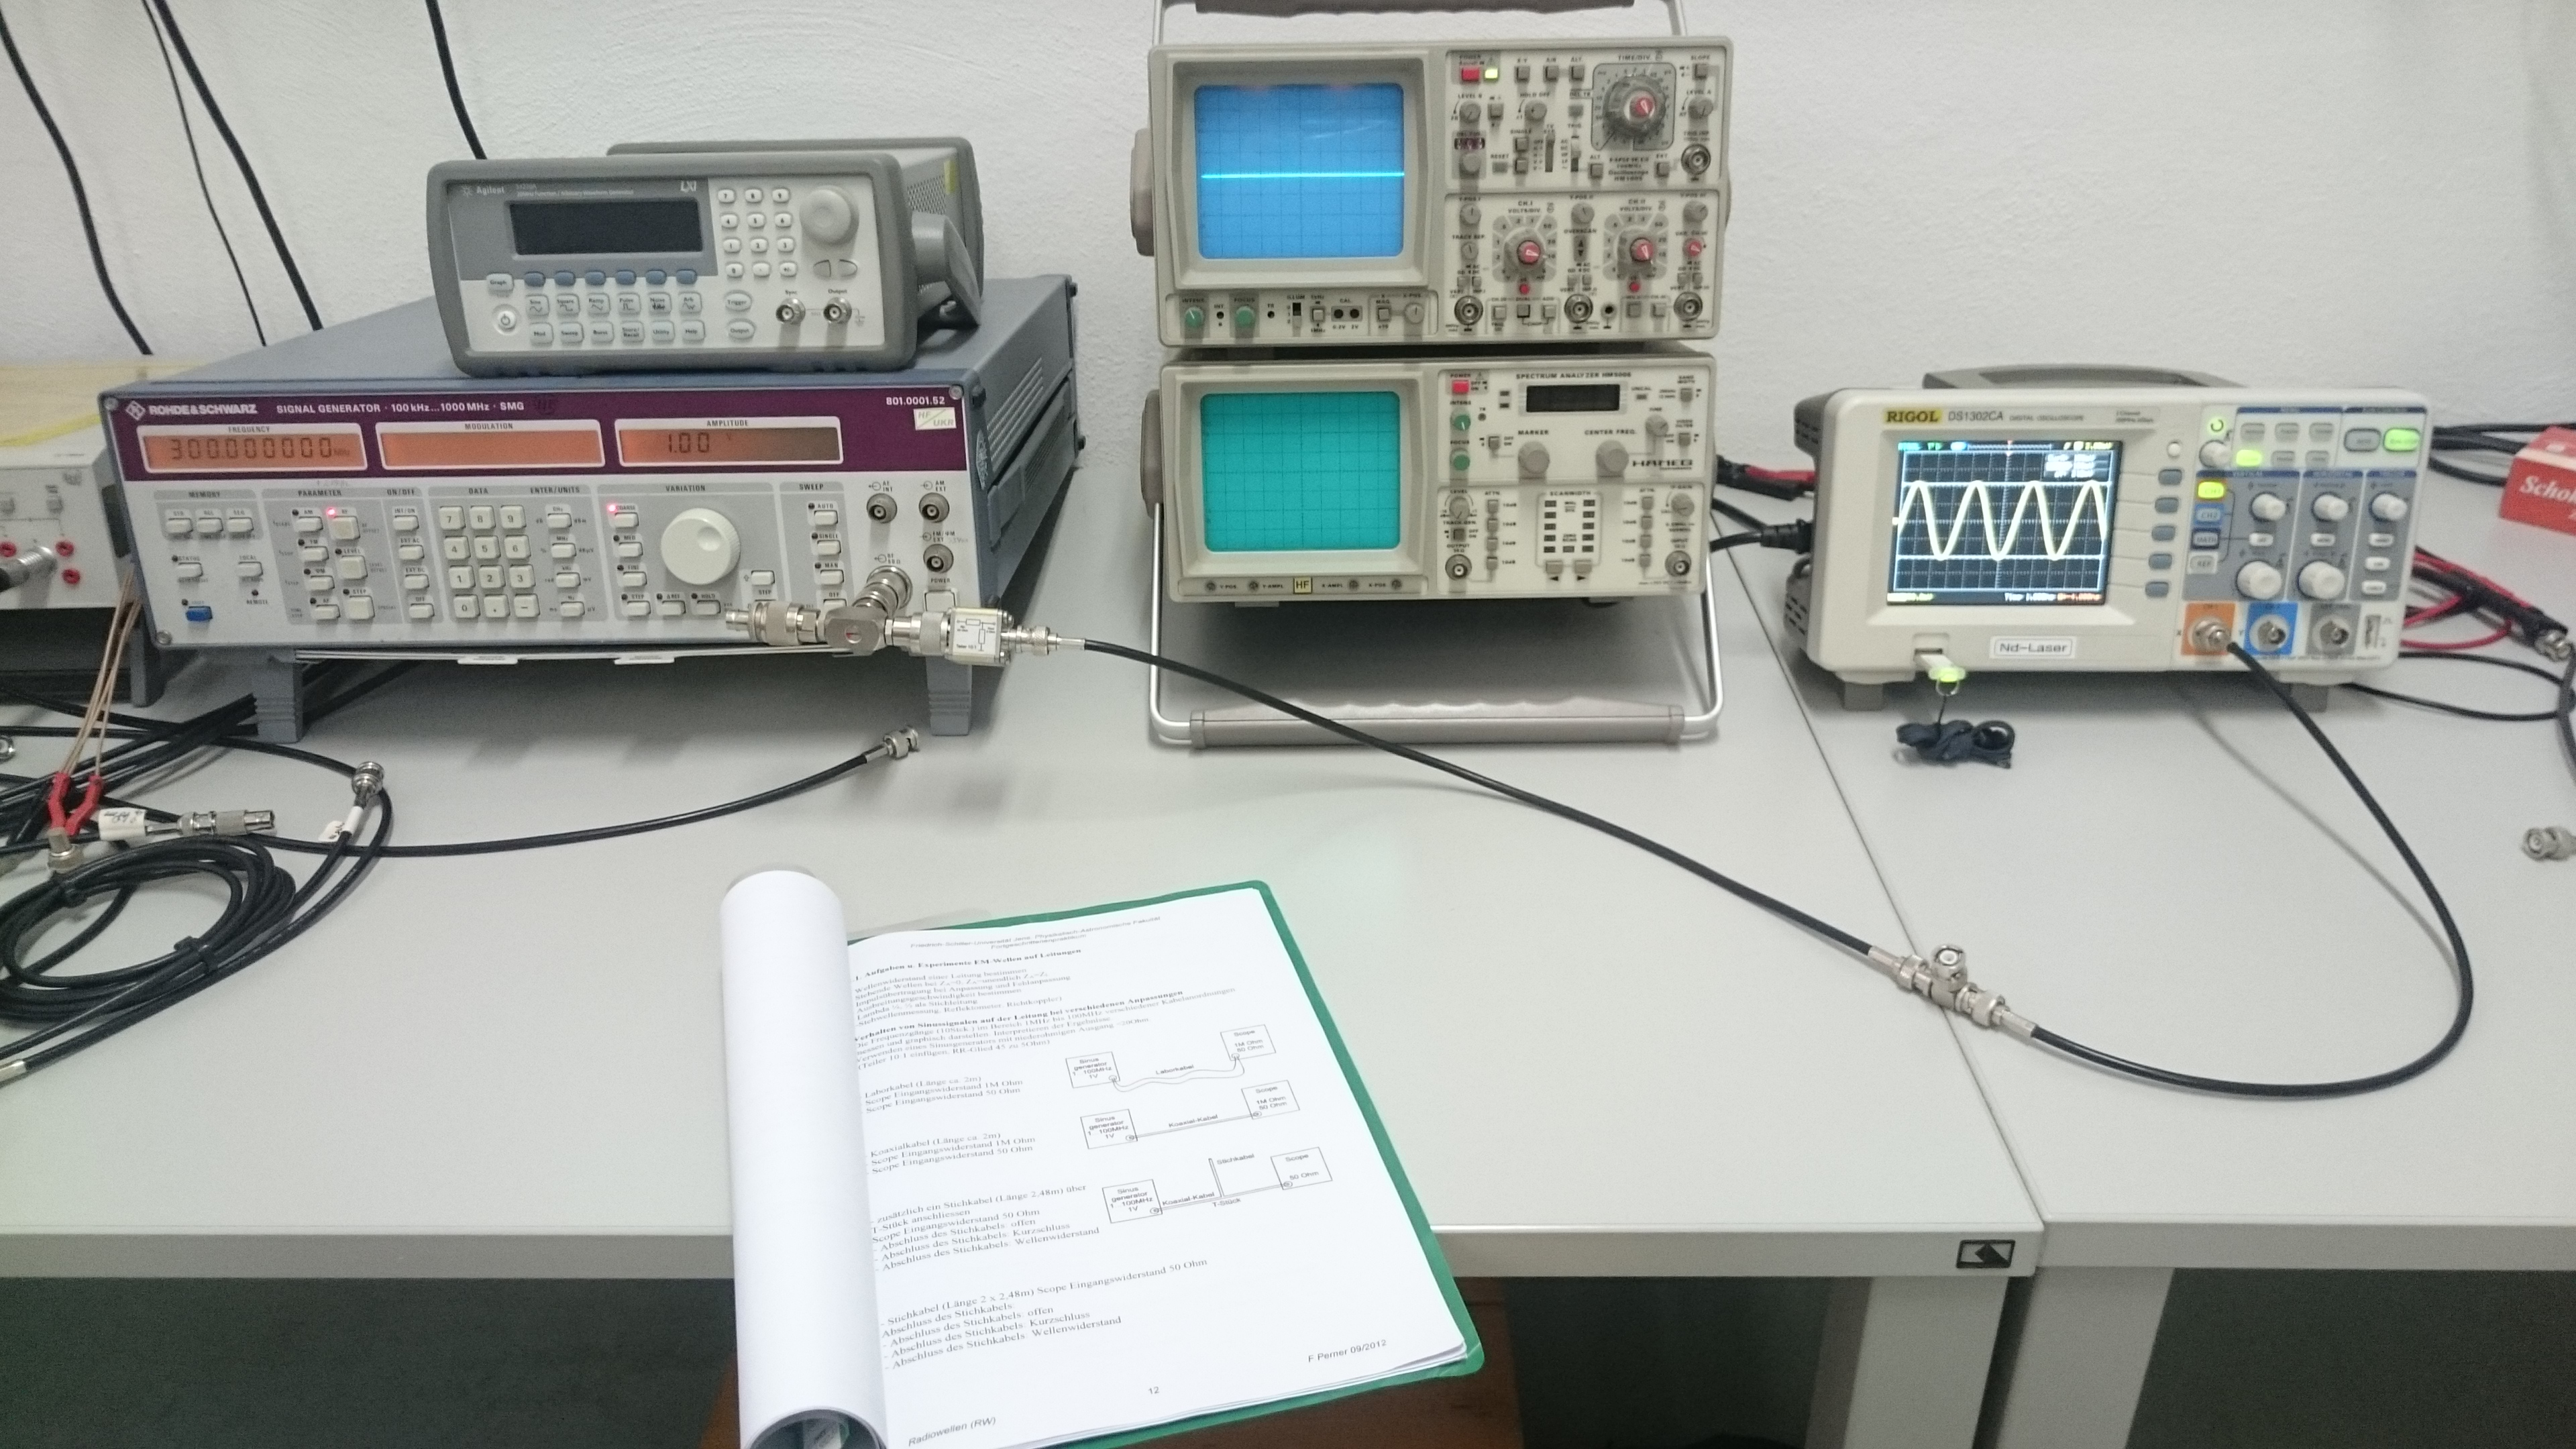
\includegraphics[scale = 0.09]{messwerte/DSC_0552.JPG}
			\caption{\centering Aufnahme des genauen Versuchsaufbaus der Koaxialkabel} %fick dich schröter
			\label{versuchsaufbau_koaxialkabel}
		\end{figure}

		In diesem Falle hatte die Lage des Kabels keinen Einfluss auf die gemessene Übertragungsfunktion.
		Diese Tatsache bestätigt die oben gegebene Begründung für die starke Abhängigkeit des Spannungsverlaufs von der Lage des Laborkabels.
		Die Spannungskurven für verschiedene Eingangswiderstände sind in der folgenden Abbildung \ref{diagramm_koaxkabel} nun genauer dargestellt.

		\begin{figure}[H]
			\center
			% GNUPLOT: LaTeX picture with Postscript
\begingroup
  \makeatletter
  \providecommand\color[2][]{%
    \GenericError{(gnuplot) \space\space\space\@spaces}{%
      Package color not loaded in conjunction with
      terminal option `colourtext'%
    }{See the gnuplot documentation for explanation.%
    }{Either use 'blacktext' in gnuplot or load the package
      color.sty in LaTeX.}%
    \renewcommand\color[2][]{}%
  }%
  \providecommand\includegraphics[2][]{%
    \GenericError{(gnuplot) \space\space\space\@spaces}{%
      Package graphicx or graphics not loaded%
    }{See the gnuplot documentation for explanation.%
    }{The gnuplot epslatex terminal needs graphicx.sty or graphics.sty.}%
    \renewcommand\includegraphics[2][]{}%
  }%
  \providecommand\rotatebox[2]{#2}%
  \@ifundefined{ifGPcolor}{%
    \newif\ifGPcolor
    \GPcolorfalse
  }{}%
  \@ifundefined{ifGPblacktext}{%
    \newif\ifGPblacktext
    \GPblacktexttrue
  }{}%
  % define a \g@addto@macro without @ in the name:
  \let\gplgaddtomacro\g@addto@macro
  % define empty templates for all commands taking text:
  \gdef\gplbacktext{}%
  \gdef\gplfronttext{}%
  \makeatother
  \ifGPblacktext
    % no textcolor at all
    \def\colorrgb#1{}%
    \def\colorgray#1{}%
  \else
    % gray or color?
    \ifGPcolor
      \def\colorrgb#1{\color[rgb]{#1}}%
      \def\colorgray#1{\color[gray]{#1}}%
      \expandafter\def\csname LTw\endcsname{\color{white}}%
      \expandafter\def\csname LTb\endcsname{\color{black}}%
      \expandafter\def\csname LTa\endcsname{\color{black}}%
      \expandafter\def\csname LT0\endcsname{\color[rgb]{1,0,0}}%
      \expandafter\def\csname LT1\endcsname{\color[rgb]{0,1,0}}%
      \expandafter\def\csname LT2\endcsname{\color[rgb]{0,0,1}}%
      \expandafter\def\csname LT3\endcsname{\color[rgb]{1,0,1}}%
      \expandafter\def\csname LT4\endcsname{\color[rgb]{0,1,1}}%
      \expandafter\def\csname LT5\endcsname{\color[rgb]{1,1,0}}%
      \expandafter\def\csname LT6\endcsname{\color[rgb]{0,0,0}}%
      \expandafter\def\csname LT7\endcsname{\color[rgb]{1,0.3,0}}%
      \expandafter\def\csname LT8\endcsname{\color[rgb]{0.5,0.5,0.5}}%
    \else
      % gray
      \def\colorrgb#1{\color{black}}%
      \def\colorgray#1{\color[gray]{#1}}%
      \expandafter\def\csname LTw\endcsname{\color{white}}%
      \expandafter\def\csname LTb\endcsname{\color{black}}%
      \expandafter\def\csname LTa\endcsname{\color{black}}%
      \expandafter\def\csname LT0\endcsname{\color{black}}%
      \expandafter\def\csname LT1\endcsname{\color{black}}%
      \expandafter\def\csname LT2\endcsname{\color{black}}%
      \expandafter\def\csname LT3\endcsname{\color{black}}%
      \expandafter\def\csname LT4\endcsname{\color{black}}%
      \expandafter\def\csname LT5\endcsname{\color{black}}%
      \expandafter\def\csname LT6\endcsname{\color{black}}%
      \expandafter\def\csname LT7\endcsname{\color{black}}%
      \expandafter\def\csname LT8\endcsname{\color{black}}%
    \fi
  \fi
  \setlength{\unitlength}{0.0500bp}%
  \begin{picture}(7370.00,3968.00)%
    \gplgaddtomacro\gplbacktext{%
      \csname LTb\endcsname%
      \put(1078,954){\makebox(0,0)[r]{\strut{} 200}}%
      \put(1078,1454){\makebox(0,0)[r]{\strut{} 400}}%
      \put(1078,1954){\makebox(0,0)[r]{\strut{} 600}}%
      \put(1078,2453){\makebox(0,0)[r]{\strut{} 800}}%
      \put(1078,2953){\makebox(0,0)[r]{\strut{} 1000}}%
      \put(1078,3453){\makebox(0,0)[r]{\strut{} 1200}}%
      \put(1210,484){\makebox(0,0){\strut{} 0}}%
      \put(2171,484){\makebox(0,0){\strut{} 50}}%
      \put(3131,484){\makebox(0,0){\strut{} 100}}%
      \put(4092,484){\makebox(0,0){\strut{} 150}}%
      \put(5052,484){\makebox(0,0){\strut{} 200}}%
      \put(6013,484){\makebox(0,0){\strut{} 250}}%
      \put(6973,484){\makebox(0,0){\strut{} 300}}%
      \put(176,2203){\rotatebox{-270}{\makebox(0,0){\strut{}$U_{pp}$ \ [mV]}}}%
      \put(4091,154){\makebox(0,0){\strut{}$f$ \ [MHz]}}%
    }%
    \gplgaddtomacro\gplfronttext{%
      \csname LTb\endcsname%
      \put(5986,3530){\makebox(0,0)[r]{\strut{}Messwerte mit $R_{in} = 50\Omega$}}%
      \csname LTb\endcsname%
      \put(5986,3310){\makebox(0,0)[r]{\strut{}Messwerte mit $R_{in} = 1$M$\Omega$}}%
    }%
    \gplbacktext
    \put(0,0){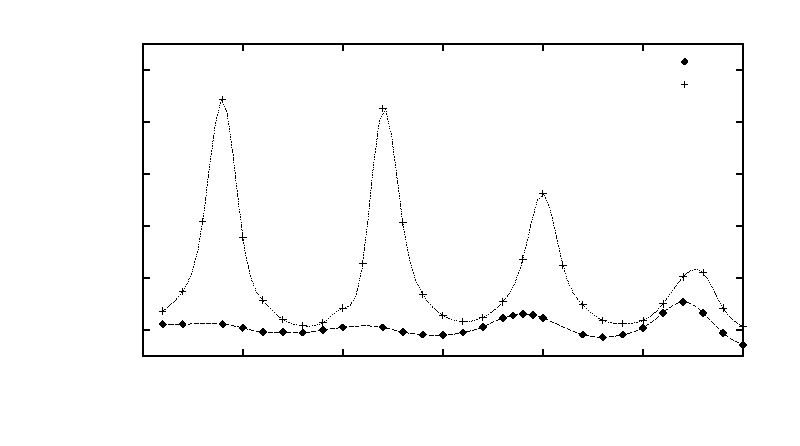
\includegraphics{koaxkabel}}%
    \gplfronttext
  \end{picture}%
\endgroup

			\caption{\centering gemessene Übertragungsfunktion des Koaxialkabels: Peak-to-Peak-Spannung $U_{pp}$ über Frequenz $f$ bei verwendetem Eingangswiderstand $R_{in}$ am Oszilloskop} %fick dich schröter
			\label{diagramm_koaxkabel}
		\end{figure}

		In diesem Kurvenverlauf wird nun deutlich, weshalb die Übertragungsfunktion für verschiedene Eingangswiderstände des Oszilloskops aufgenommen wurde.
		Für einen Eingangswiderstand von $1$M$\Omega$ ist immer noch eine starke Änderung der Peak-to-Peak-Spannung beobachtbar.
		Dennoch scheint das Signal hier regelmäßig zu variieren. 
		Maxima tauchen, wie man im Diagramm sehen kann, immer bei ungeradzahligen Vielfachen von ungefähr $40$MHz auf, wie zum Beispiel bei $40$MHz, $120$MHz oder $200$MHz.
		Dagegen entstehen Minima immer bei geradzahligen Vielfachen.
		Dies deutet darauf hin, dass es im Kabel zur Ausbildung von stehenden Wellen kommt, wodurch je nach Länge des Kabels an dessen Ende immer wieder Maxima und Minima an bestimmten Stellen gemessen werden können.
		Stehende Wellen können aber nur entstehen, wenn das gesendete Signal am Eingang des Oszilloskops wieder reflektiert wird (siehe Grundlagen).
		Wie aus den Grundlagen bekannt ist, kann die Reflexion durch eine Anpassung des Eingangswiderstand mit dem Wellenwiderstand minimiert wenn nicht sogar verhindert werden.
		Der Wellenwiderstand beträgt wie oben erwähnt nun $50\Omega$.
		Es ist also zu erwarten, dass sich für einen Eingangswiderstand von $50\Omega$ keine stehenden Wellen mehr ausbilden.
		Betrachtet man mit diesen Gedanken das Diagramm \ref{diagramm_koaxkabel}, so erklärt sich der fast konstante Verlauf der Kurve mit geringerem Eingangswiderstand.
		Kleinere Abweichungen für größere Frequenzen sind nicht zu vermeiden, da eine unendliche genaue Anpassung des Eingangswiderstands nicht möglich ist. \\

		Demzufolge ist eine Anpassung der Widerstände an den Wellenwiderstand des Kabels notwendig, um einen halbwegs konstanten Spannungsverlauf zu gewährleisten.
		Aus diesem Grund wurden fortan alle weiteren Messungen, wenn nicht anders angegeben, mit einem Eingangswiderstand von $50\Omega$ aufgenommen. 

	% subsubsection koaxialkabel (end)

	\subsubsection{Koaxialkabel mit eingefügtem Stichkabel} % (fold)
	\label{ssub:koaxialkabel_mit_eingef_gtem_stichkabel}

		Für eine genauere Untersuchung der sich ausbildenden stehenden Wellen, soll nun oben verwendetes Kabel mit einem weiteren Koaxialkabel versehen werden, welches Stichkabel genannt wird.
		Dieses Kabel wurde mithilfe eines T-Stücks befestigt.
		Es besitzt eine Länge von $2.48$m.
		In der Aufnahme \ref{versuchsaufbau_stichkabel} wird dies genauer gezeigt.
		Aufgrund des angepassten Eingangswiderstandes sind entlang des alten Kabels keine stehenden Wellen zu erwarten.

		\begin{figure}[H]
			\center
			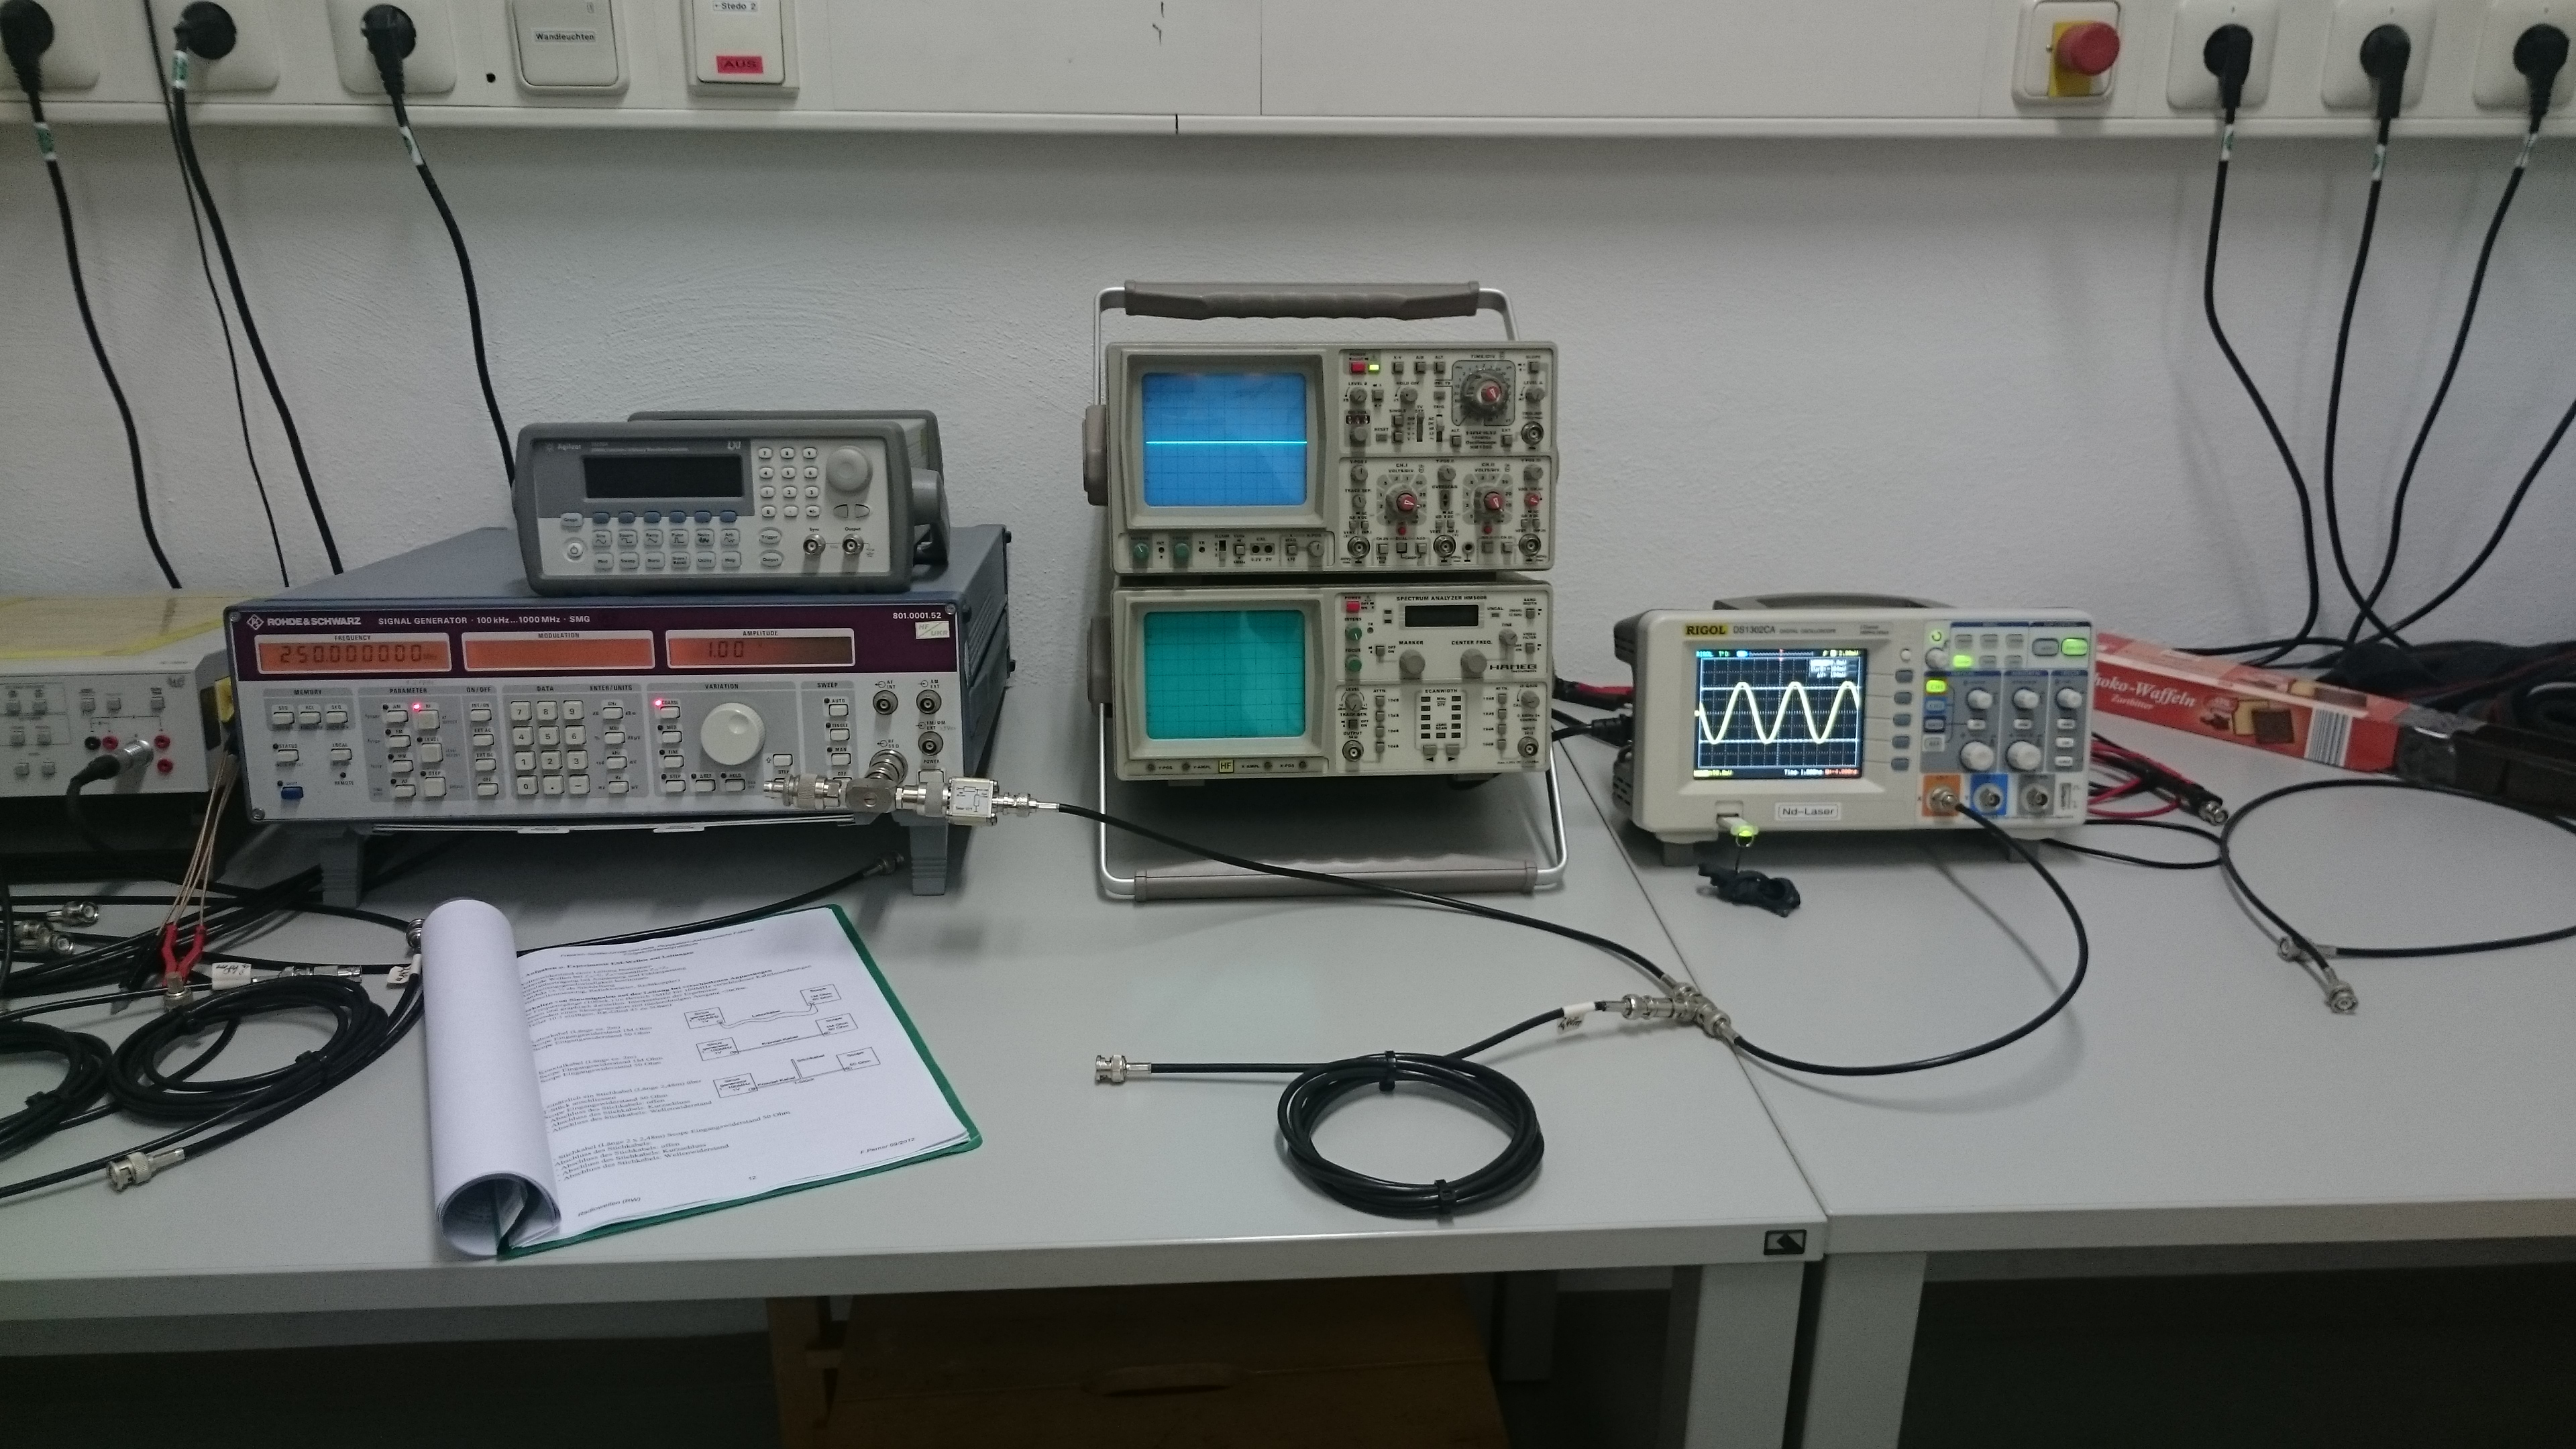
\includegraphics[scale = 0.09]{messwerte/DSC_0553.JPG}
			\caption{\centering Aufnahme des genauen Versuchsaufbaus des Koaxialkabels mit eingestecktem Stichkabel} %fick dich schröter
			\label{versuchsaufbau_stichkabel}
		\end{figure}

		Der Spannungsverlauf selbst sollte nun für drei verschiedene Fälle aufgenommen werden.
		Im ersten Fall wurde das Kabel am Ende offen gelassen.
		Im Falle eines Gleichstromes würde also durch das Stichkabel überhaupt kein Strom fließen.
		In der gemessenen Übertragungsfunktion in Abbildung \ref{diagramm_stichkabel_offen} ist nun aber eine klare Variation der Spannung zu sehen.

		\begin{figure}[H]
			\center
			% GNUPLOT: LaTeX picture with Postscript
\begingroup
  \makeatletter
  \providecommand\color[2][]{%
    \GenericError{(gnuplot) \space\space\space\@spaces}{%
      Package color not loaded in conjunction with
      terminal option `colourtext'%
    }{See the gnuplot documentation for explanation.%
    }{Either use 'blacktext' in gnuplot or load the package
      color.sty in LaTeX.}%
    \renewcommand\color[2][]{}%
  }%
  \providecommand\includegraphics[2][]{%
    \GenericError{(gnuplot) \space\space\space\@spaces}{%
      Package graphicx or graphics not loaded%
    }{See the gnuplot documentation for explanation.%
    }{The gnuplot epslatex terminal needs graphicx.sty or graphics.sty.}%
    \renewcommand\includegraphics[2][]{}%
  }%
  \providecommand\rotatebox[2]{#2}%
  \@ifundefined{ifGPcolor}{%
    \newif\ifGPcolor
    \GPcolorfalse
  }{}%
  \@ifundefined{ifGPblacktext}{%
    \newif\ifGPblacktext
    \GPblacktexttrue
  }{}%
  % define a \g@addto@macro without @ in the name:
  \let\gplgaddtomacro\g@addto@macro
  % define empty templates for all commands taking text:
  \gdef\gplbacktext{}%
  \gdef\gplfronttext{}%
  \makeatother
  \ifGPblacktext
    % no textcolor at all
    \def\colorrgb#1{}%
    \def\colorgray#1{}%
  \else
    % gray or color?
    \ifGPcolor
      \def\colorrgb#1{\color[rgb]{#1}}%
      \def\colorgray#1{\color[gray]{#1}}%
      \expandafter\def\csname LTw\endcsname{\color{white}}%
      \expandafter\def\csname LTb\endcsname{\color{black}}%
      \expandafter\def\csname LTa\endcsname{\color{black}}%
      \expandafter\def\csname LT0\endcsname{\color[rgb]{1,0,0}}%
      \expandafter\def\csname LT1\endcsname{\color[rgb]{0,1,0}}%
      \expandafter\def\csname LT2\endcsname{\color[rgb]{0,0,1}}%
      \expandafter\def\csname LT3\endcsname{\color[rgb]{1,0,1}}%
      \expandafter\def\csname LT4\endcsname{\color[rgb]{0,1,1}}%
      \expandafter\def\csname LT5\endcsname{\color[rgb]{1,1,0}}%
      \expandafter\def\csname LT6\endcsname{\color[rgb]{0,0,0}}%
      \expandafter\def\csname LT7\endcsname{\color[rgb]{1,0.3,0}}%
      \expandafter\def\csname LT8\endcsname{\color[rgb]{0.5,0.5,0.5}}%
    \else
      % gray
      \def\colorrgb#1{\color{black}}%
      \def\colorgray#1{\color[gray]{#1}}%
      \expandafter\def\csname LTw\endcsname{\color{white}}%
      \expandafter\def\csname LTb\endcsname{\color{black}}%
      \expandafter\def\csname LTa\endcsname{\color{black}}%
      \expandafter\def\csname LT0\endcsname{\color{black}}%
      \expandafter\def\csname LT1\endcsname{\color{black}}%
      \expandafter\def\csname LT2\endcsname{\color{black}}%
      \expandafter\def\csname LT3\endcsname{\color{black}}%
      \expandafter\def\csname LT4\endcsname{\color{black}}%
      \expandafter\def\csname LT5\endcsname{\color{black}}%
      \expandafter\def\csname LT6\endcsname{\color{black}}%
      \expandafter\def\csname LT7\endcsname{\color{black}}%
      \expandafter\def\csname LT8\endcsname{\color{black}}%
    \fi
  \fi
  \setlength{\unitlength}{0.0500bp}%
  \begin{picture}(7370.00,3968.00)%
    \gplgaddtomacro\gplbacktext{%
      \csname LTb\endcsname%
      \put(946,704){\makebox(0,0)[r]{\strut{} 0}}%
      \put(946,1132){\makebox(0,0)[r]{\strut{} 50}}%
      \put(946,1561){\makebox(0,0)[r]{\strut{} 100}}%
      \put(946,1989){\makebox(0,0)[r]{\strut{} 150}}%
      \put(946,2418){\makebox(0,0)[r]{\strut{} 200}}%
      \put(946,2846){\makebox(0,0)[r]{\strut{} 250}}%
      \put(946,3275){\makebox(0,0)[r]{\strut{} 300}}%
      \put(946,3703){\makebox(0,0)[r]{\strut{} 350}}%
      \put(1078,484){\makebox(0,0){\strut{} 0}}%
      \put(2061,484){\makebox(0,0){\strut{} 50}}%
      \put(3043,484){\makebox(0,0){\strut{} 100}}%
      \put(4026,484){\makebox(0,0){\strut{} 150}}%
      \put(5008,484){\makebox(0,0){\strut{} 200}}%
      \put(5991,484){\makebox(0,0){\strut{} 250}}%
      \put(6973,484){\makebox(0,0){\strut{} 300}}%
      \put(176,2203){\rotatebox{-270}{\makebox(0,0){\strut{}$U_{pp}$ \ [mV]}}}%
      \put(4025,154){\makebox(0,0){\strut{}$f$ \ [MHz]}}%
    }%
    \gplgaddtomacro\gplfronttext{%
      \csname LTb\endcsname%
      \put(5986,3530){\makebox(0,0)[r]{\strut{}Messwerte}}%
    }%
    \gplbacktext
    \put(0,0){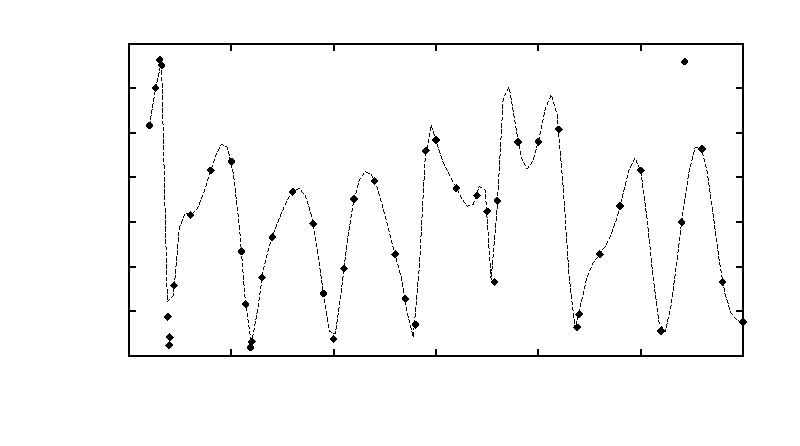
\includegraphics{stichkabel-01}}%
    \gplfronttext
  \end{picture}%
\endgroup

			\caption{\centering gemessene Übertragungsfunktion des Koaxialkabels mit offenem Stichkabel: Peak-to-Peak-Spannung $U_{pp}$ über Frequenz $f$} %fick dich schröter
			\label{diagramm_stichkabel_offen}
		\end{figure}

		Auch hier tauchen Maxima und Minima sehr regelmäßig auf, was, wie zu erwarten war, wieder auf stehende Wellen im Stichkabel zurückzuführen ist.
		Aufgrund der in den Grundlagen betrachteten Theorie zu stehenden Wellen in Leitungen ist klar, dass am offenen Ende des Stichkabels die Spannung immer maximal sein muss, damit sich stehende Wellen ausbilden.
		Die Minima in der Übertragungsfunktion entstehen nun dadurch, dass sich am T-Stück ein Knotenpunkt des Spannungsverlaufs bildet.
		Für einen Knoten muss die Spannung hier also auf Null oder zumindest auf ein Minimum fallen.
		Folgende Darstellung soll dies veranschaulichen:

		\begin{figure}[H]
			\center
			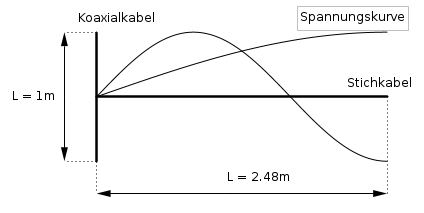
\includegraphics[scale = 0.8]{schema-02.png}
			\caption{\centering schematische Darstellung zur Erklärung der Entstehung von stehenden Wellen im offenen Stichkabel}
			\label{schema-stehende-welle}
		\end{figure}

		Die Abbildung \ref{schema-stehende-welle} macht noch einmal die Ausbildung von stehenden Wellen deutlich.
		Die maximale Wellenlänge der stehenden Welle im Stichkabel mit Länge $L$ ist also $4L$ oder auch $9.92$m.
		Demnach entsteht genau dann eine stehende Welle mit Wellenlänge $\lambda$ und den betrachteten Eigenschaften im Stichkabel mit Länge $L$, wenn es ein $n \in \mathbb{N}$ gibt, sodass gilt:
		\begin{equation}
			(2n-1)\dfrac{\lambda}{4} = L
		\end{equation}
		Mit dieser Formel und der Gleichung $c = f\cdot \lambda$, wobei $c$ die Geschwindigkeit der Welle im Stichkabel ist und $f$ deren Frequenz, folgt nun:
		\begin{equation}
			f = (2n-1)\dfrac{c}{4L}
		\end{equation}
		Das erste Minimum (also $n=1$) wurde für $f = 19.7$MHz gemessen.
		Damit ergibt sich der Verkürzungsfaktor $K$ des Kabels zu:
		\[
			K = \dfrac{c}{c_0} = \dfrac{4Lf}{c_0} = \dfrac{4\cdot 2.48\text{m} \cdot 19.7\text{MHz}}{3\cdot 10^8\text{ms}^{-1}} \approx 0.65
		\]
		\[
			c = K\cdot c_0 = 4Lf = 4\cdot 2.48\text{m} \cdot 19.7\text{MHz} \approx 1.954\cdot 10^8\text{ms}^{-1}
		\]
		Demzufolge müssten sich weitere Minima bei $59.1$MHz, $98.5$MHz, $137.9$MHz, $177.3$MHz usw. befinden.
		Dies lässt sich anhand des Kurvenverlaufs in Abbildung \ref{diagramm_koaxkabel} bestätigen.

		Im zweiten Fall sollte das Stichkabel kurzgeschlossen werden.
		Analog zu den obigen Betrachtungen muss sich auch hier ein Minimum am Knotenpunkt ausbilden, damit ein Minimum im Spannungsverlauf sichtbar wird.
		Anhand der Grundlagen ist klar, dass sich für stehende Wellen am kurzgeschlossenen Ende des Stichkabels nur ein weiterer Knotenpunkt befinden darf.
		Es muss damit folgende Bedingung für eine stehende Welle mit der Wellenlänge $\lambda$ im Stichkabel der Länge $L$ gelten:
		\begin{equation}
			\dfrac{n\lambda}{2} = L \qquad \text{für ein $n \in \mathbb{N}$}
		\end{equation}
		\begin{equation}
			f = n\dfrac{c}{2L}
		\end{equation}
		Die gemessene Übertragungsfunktion des geschlossenen Stichkabels ist in Abbildung \ref{diagramm_stichkabel_geschlossen} aufgetragen.

		\begin{figure}[H]
			\center
			% GNUPLOT: LaTeX picture with Postscript
\begingroup
  \makeatletter
  \providecommand\color[2][]{%
    \GenericError{(gnuplot) \space\space\space\@spaces}{%
      Package color not loaded in conjunction with
      terminal option `colourtext'%
    }{See the gnuplot documentation for explanation.%
    }{Either use 'blacktext' in gnuplot or load the package
      color.sty in LaTeX.}%
    \renewcommand\color[2][]{}%
  }%
  \providecommand\includegraphics[2][]{%
    \GenericError{(gnuplot) \space\space\space\@spaces}{%
      Package graphicx or graphics not loaded%
    }{See the gnuplot documentation for explanation.%
    }{The gnuplot epslatex terminal needs graphicx.sty or graphics.sty.}%
    \renewcommand\includegraphics[2][]{}%
  }%
  \providecommand\rotatebox[2]{#2}%
  \@ifundefined{ifGPcolor}{%
    \newif\ifGPcolor
    \GPcolorfalse
  }{}%
  \@ifundefined{ifGPblacktext}{%
    \newif\ifGPblacktext
    \GPblacktexttrue
  }{}%
  % define a \g@addto@macro without @ in the name:
  \let\gplgaddtomacro\g@addto@macro
  % define empty templates for all commands taking text:
  \gdef\gplbacktext{}%
  \gdef\gplfronttext{}%
  \makeatother
  \ifGPblacktext
    % no textcolor at all
    \def\colorrgb#1{}%
    \def\colorgray#1{}%
  \else
    % gray or color?
    \ifGPcolor
      \def\colorrgb#1{\color[rgb]{#1}}%
      \def\colorgray#1{\color[gray]{#1}}%
      \expandafter\def\csname LTw\endcsname{\color{white}}%
      \expandafter\def\csname LTb\endcsname{\color{black}}%
      \expandafter\def\csname LTa\endcsname{\color{black}}%
      \expandafter\def\csname LT0\endcsname{\color[rgb]{1,0,0}}%
      \expandafter\def\csname LT1\endcsname{\color[rgb]{0,1,0}}%
      \expandafter\def\csname LT2\endcsname{\color[rgb]{0,0,1}}%
      \expandafter\def\csname LT3\endcsname{\color[rgb]{1,0,1}}%
      \expandafter\def\csname LT4\endcsname{\color[rgb]{0,1,1}}%
      \expandafter\def\csname LT5\endcsname{\color[rgb]{1,1,0}}%
      \expandafter\def\csname LT6\endcsname{\color[rgb]{0,0,0}}%
      \expandafter\def\csname LT7\endcsname{\color[rgb]{1,0.3,0}}%
      \expandafter\def\csname LT8\endcsname{\color[rgb]{0.5,0.5,0.5}}%
    \else
      % gray
      \def\colorrgb#1{\color{black}}%
      \def\colorgray#1{\color[gray]{#1}}%
      \expandafter\def\csname LTw\endcsname{\color{white}}%
      \expandafter\def\csname LTb\endcsname{\color{black}}%
      \expandafter\def\csname LTa\endcsname{\color{black}}%
      \expandafter\def\csname LT0\endcsname{\color{black}}%
      \expandafter\def\csname LT1\endcsname{\color{black}}%
      \expandafter\def\csname LT2\endcsname{\color{black}}%
      \expandafter\def\csname LT3\endcsname{\color{black}}%
      \expandafter\def\csname LT4\endcsname{\color{black}}%
      \expandafter\def\csname LT5\endcsname{\color{black}}%
      \expandafter\def\csname LT6\endcsname{\color{black}}%
      \expandafter\def\csname LT7\endcsname{\color{black}}%
      \expandafter\def\csname LT8\endcsname{\color{black}}%
    \fi
  \fi
  \setlength{\unitlength}{0.0500bp}%
  \begin{picture}(7370.00,3968.00)%
    \gplgaddtomacro\gplbacktext{%
      \csname LTb\endcsname%
      \put(946,704){\makebox(0,0)[r]{\strut{} 0}}%
      \put(946,1132){\makebox(0,0)[r]{\strut{} 50}}%
      \put(946,1561){\makebox(0,0)[r]{\strut{} 100}}%
      \put(946,1989){\makebox(0,0)[r]{\strut{} 150}}%
      \put(946,2418){\makebox(0,0)[r]{\strut{} 200}}%
      \put(946,2846){\makebox(0,0)[r]{\strut{} 250}}%
      \put(946,3275){\makebox(0,0)[r]{\strut{} 300}}%
      \put(946,3703){\makebox(0,0)[r]{\strut{} 350}}%
      \put(1078,484){\makebox(0,0){\strut{} 0}}%
      \put(2061,484){\makebox(0,0){\strut{} 50}}%
      \put(3043,484){\makebox(0,0){\strut{} 100}}%
      \put(4026,484){\makebox(0,0){\strut{} 150}}%
      \put(5008,484){\makebox(0,0){\strut{} 200}}%
      \put(5991,484){\makebox(0,0){\strut{} 250}}%
      \put(6973,484){\makebox(0,0){\strut{} 300}}%
      \put(176,2203){\rotatebox{-270}{\makebox(0,0){\strut{}$U_{pp}$ \ [mV]}}}%
      \put(4025,154){\makebox(0,0){\strut{}$f$ \ [MHz]}}%
    }%
    \gplgaddtomacro\gplfronttext{%
      \csname LTb\endcsname%
      \put(5986,3530){\makebox(0,0)[r]{\strut{}Messwerte}}%
    }%
    \gplbacktext
    \put(0,0){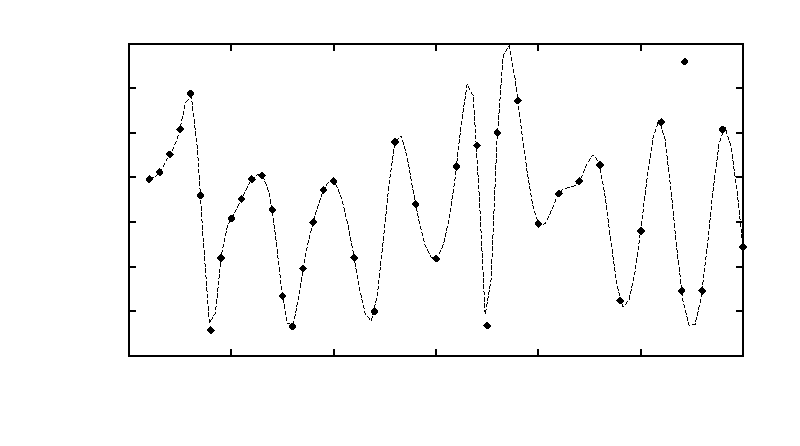
\includegraphics{stichkabel-02}}%
    \gplfronttext
  \end{picture}%
\endgroup

			\caption{\centering gemessene Übertragungsfunktion des Koaxialkabels mit kurzgeschlossenem Stichkabel: Peak-to-Peak-Spannung $U_{pp}$ über Frequenz $f$} %fick dich schröter
			\label{diagramm_stichkabel_geschlossen}
		\end{figure}

		Hier ist ein ganz ähnliches Verhalten wie vorher zu beobachten.
		Minima und Maxima tauchen wieder im gleichen Abstand auf.
		Auch dies deckt sich mit der bisherigen Theorie.
		Das erste Minimum (also $n = 1$) wurde dieses Mal jedoch bei $f = 38$MHz gemessen.
		Analog zur obigen Rechnung ergibt sich nun der Verkürzungsfaktor $K$ zu:
		\[
			K \approx 0.63
		\]
		\[
			c \approx 1.885\cdot 10^8\text{ms}^{-1}
		\]
		Der Verkürzungsfaktor sollte unabhängig von der jeweiligen verwendeten Schaltung sein.
		Die Differenz liegt hier im Bereich der bisherigen relativen Fehler (in etwa $10$ bis $20$\%) und kann damit als konstant gesehen werden.
		Ähnlich zu oben sind die Minima hier bei $38$MHz, $76$MHz, $114$MHz usw. zu erwarten.
		Die Kurve bestätigt auch hier die Theorie.

		Im letzten Fall wurde auf das Ende des Stichkabels ein ohmscher Widerstand von $50\Omega$ geschraubt.
		Dies entspricht damit gerade der Anpassungsbedingung.
		Abbildung \ref{diagramm_stichkabel_angepasst} zeigt die gemessene Kurve.

		\begin{figure}[H]
			\center
			% GNUPLOT: LaTeX picture with Postscript
\begingroup
  \makeatletter
  \providecommand\color[2][]{%
    \GenericError{(gnuplot) \space\space\space\@spaces}{%
      Package color not loaded in conjunction with
      terminal option `colourtext'%
    }{See the gnuplot documentation for explanation.%
    }{Either use 'blacktext' in gnuplot or load the package
      color.sty in LaTeX.}%
    \renewcommand\color[2][]{}%
  }%
  \providecommand\includegraphics[2][]{%
    \GenericError{(gnuplot) \space\space\space\@spaces}{%
      Package graphicx or graphics not loaded%
    }{See the gnuplot documentation for explanation.%
    }{The gnuplot epslatex terminal needs graphicx.sty or graphics.sty.}%
    \renewcommand\includegraphics[2][]{}%
  }%
  \providecommand\rotatebox[2]{#2}%
  \@ifundefined{ifGPcolor}{%
    \newif\ifGPcolor
    \GPcolorfalse
  }{}%
  \@ifundefined{ifGPblacktext}{%
    \newif\ifGPblacktext
    \GPblacktexttrue
  }{}%
  % define a \g@addto@macro without @ in the name:
  \let\gplgaddtomacro\g@addto@macro
  % define empty templates for all commands taking text:
  \gdef\gplbacktext{}%
  \gdef\gplfronttext{}%
  \makeatother
  \ifGPblacktext
    % no textcolor at all
    \def\colorrgb#1{}%
    \def\colorgray#1{}%
  \else
    % gray or color?
    \ifGPcolor
      \def\colorrgb#1{\color[rgb]{#1}}%
      \def\colorgray#1{\color[gray]{#1}}%
      \expandafter\def\csname LTw\endcsname{\color{white}}%
      \expandafter\def\csname LTb\endcsname{\color{black}}%
      \expandafter\def\csname LTa\endcsname{\color{black}}%
      \expandafter\def\csname LT0\endcsname{\color[rgb]{1,0,0}}%
      \expandafter\def\csname LT1\endcsname{\color[rgb]{0,1,0}}%
      \expandafter\def\csname LT2\endcsname{\color[rgb]{0,0,1}}%
      \expandafter\def\csname LT3\endcsname{\color[rgb]{1,0,1}}%
      \expandafter\def\csname LT4\endcsname{\color[rgb]{0,1,1}}%
      \expandafter\def\csname LT5\endcsname{\color[rgb]{1,1,0}}%
      \expandafter\def\csname LT6\endcsname{\color[rgb]{0,0,0}}%
      \expandafter\def\csname LT7\endcsname{\color[rgb]{1,0.3,0}}%
      \expandafter\def\csname LT8\endcsname{\color[rgb]{0.5,0.5,0.5}}%
    \else
      % gray
      \def\colorrgb#1{\color{black}}%
      \def\colorgray#1{\color[gray]{#1}}%
      \expandafter\def\csname LTw\endcsname{\color{white}}%
      \expandafter\def\csname LTb\endcsname{\color{black}}%
      \expandafter\def\csname LTa\endcsname{\color{black}}%
      \expandafter\def\csname LT0\endcsname{\color{black}}%
      \expandafter\def\csname LT1\endcsname{\color{black}}%
      \expandafter\def\csname LT2\endcsname{\color{black}}%
      \expandafter\def\csname LT3\endcsname{\color{black}}%
      \expandafter\def\csname LT4\endcsname{\color{black}}%
      \expandafter\def\csname LT5\endcsname{\color{black}}%
      \expandafter\def\csname LT6\endcsname{\color{black}}%
      \expandafter\def\csname LT7\endcsname{\color{black}}%
      \expandafter\def\csname LT8\endcsname{\color{black}}%
    \fi
  \fi
  \setlength{\unitlength}{0.0500bp}%
  \begin{picture}(7370.00,3968.00)%
    \gplgaddtomacro\gplbacktext{%
      \csname LTb\endcsname%
      \put(946,704){\makebox(0,0)[r]{\strut{} 80}}%
      \put(946,1079){\makebox(0,0)[r]{\strut{} 100}}%
      \put(946,1454){\makebox(0,0)[r]{\strut{} 120}}%
      \put(946,1829){\makebox(0,0)[r]{\strut{} 140}}%
      \put(946,2204){\makebox(0,0)[r]{\strut{} 160}}%
      \put(946,2578){\makebox(0,0)[r]{\strut{} 180}}%
      \put(946,2953){\makebox(0,0)[r]{\strut{} 200}}%
      \put(946,3328){\makebox(0,0)[r]{\strut{} 220}}%
      \put(946,3703){\makebox(0,0)[r]{\strut{} 240}}%
      \put(1078,484){\makebox(0,0){\strut{} 0}}%
      \put(2061,484){\makebox(0,0){\strut{} 50}}%
      \put(3043,484){\makebox(0,0){\strut{} 100}}%
      \put(4026,484){\makebox(0,0){\strut{} 150}}%
      \put(5008,484){\makebox(0,0){\strut{} 200}}%
      \put(5991,484){\makebox(0,0){\strut{} 250}}%
      \put(6973,484){\makebox(0,0){\strut{} 300}}%
      \put(176,2203){\rotatebox{-270}{\makebox(0,0){\strut{}$U_{pp}$ \ [mV]}}}%
      \put(4025,154){\makebox(0,0){\strut{}$f$ \ [MHz]}}%
    }%
    \gplgaddtomacro\gplfronttext{%
      \csname LTb\endcsname%
      \put(5986,3530){\makebox(0,0)[r]{\strut{}Messwerte}}%
    }%
    \gplbacktext
    \put(0,0){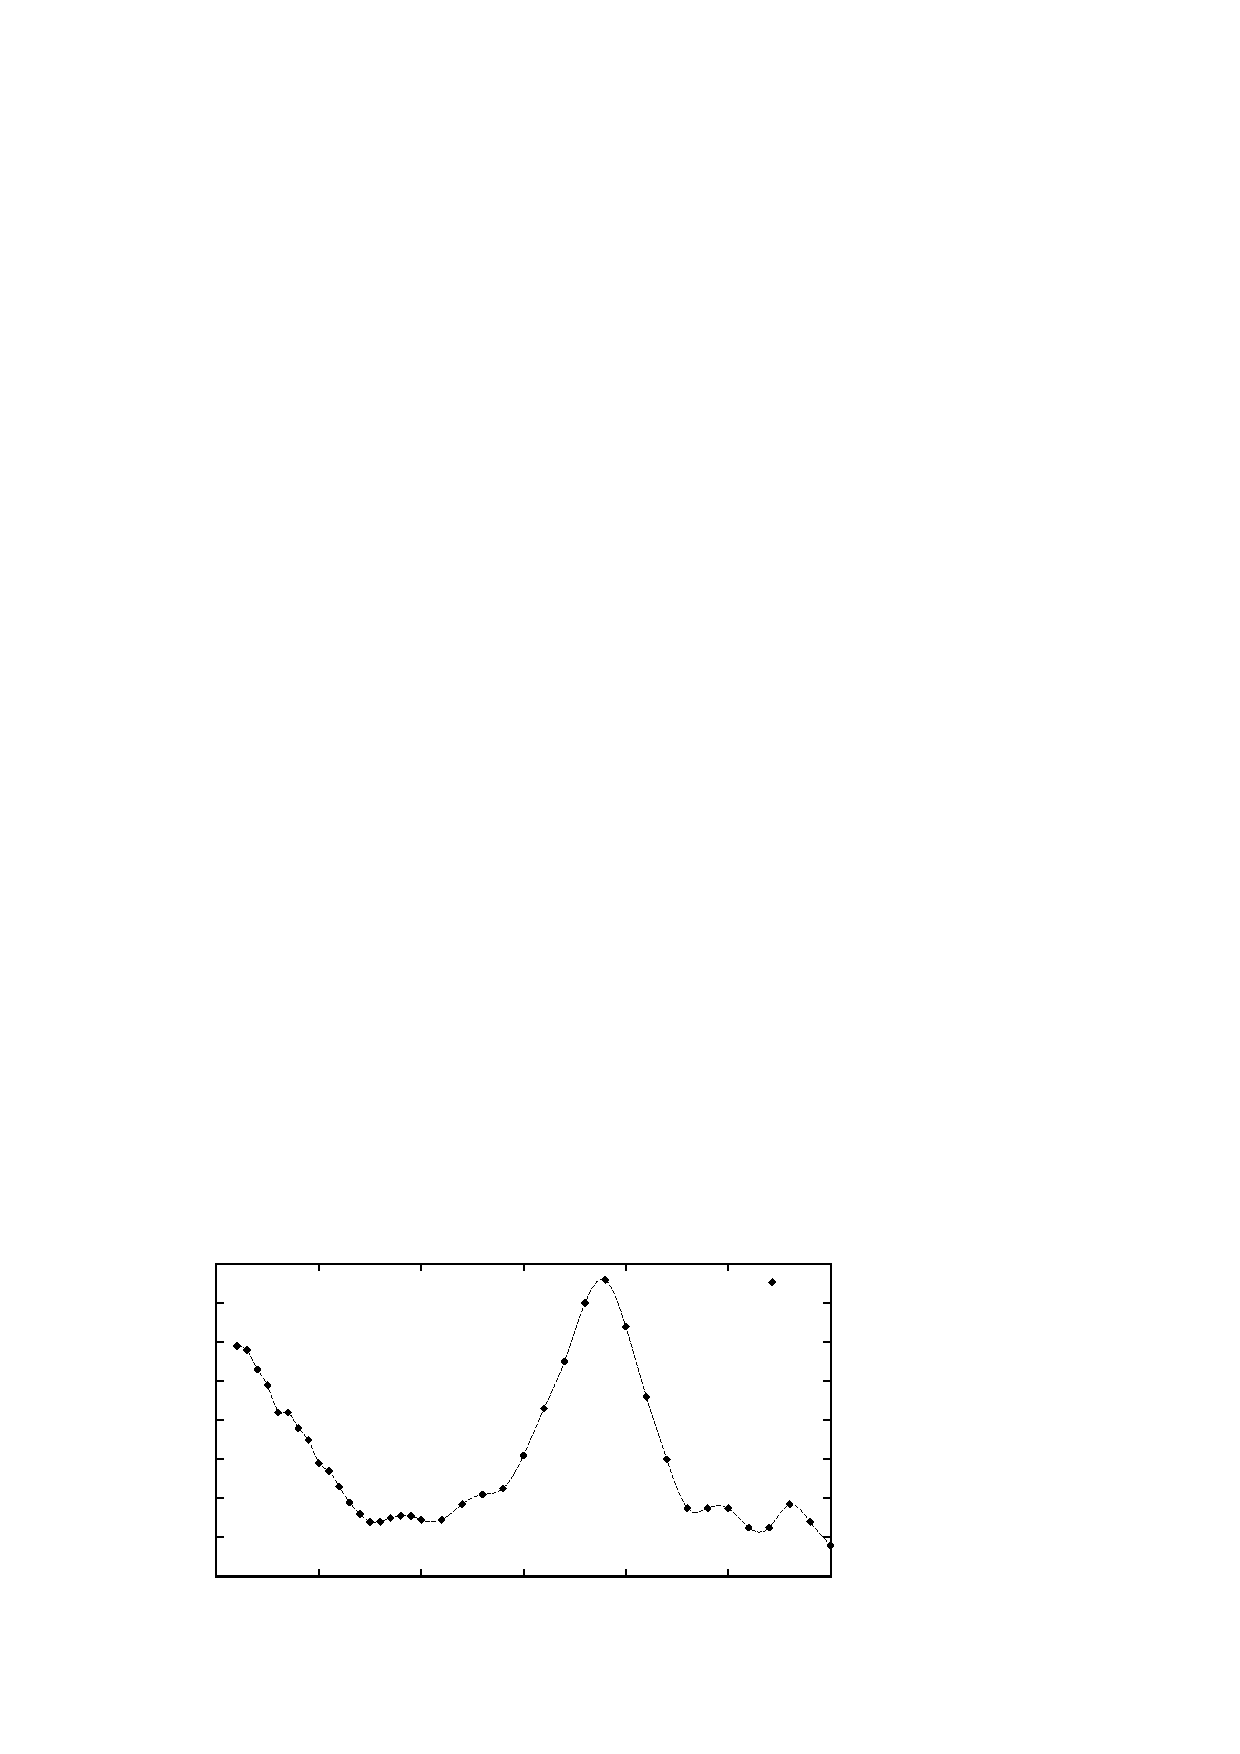
\includegraphics{stichkabel-03}}%
    \gplfronttext
  \end{picture}%
\endgroup

			\caption{\centering gemessene Übertragungsfunktion des Koaxialkabels mit angepasstem Stichkabel: Peak-to-Peak-Spannung $U_{pp}$ über Frequenz $f$} %fick dich schröter
			\label{diagramm_stichkabel_angepasst}
		\end{figure}

		Aufgrund der erfüllten Anpassungsbedingung können am Ende des Stichkabels keine stehenden Wellen entstehen.
		Dies erklärt, dass sich keine scharfen Maxima oder Minima im Graphen ausbilden.
		Die weitläufige Schwankung im Spannungsverlauf wird durch sehr geringe Unterschiede des angesteckten Widerstandes und des Wellenwiderstandes verursacht.
		Abbildung \ref{diagramm_stichkabel_alles} stellt noch einmal eine Zusammenfassung aller Graphen dar.

		\begin{figure}[H]
			\center
			% GNUPLOT: LaTeX picture with Postscript
\begingroup
  \makeatletter
  \providecommand\color[2][]{%
    \GenericError{(gnuplot) \space\space\space\@spaces}{%
      Package color not loaded in conjunction with
      terminal option `colourtext'%
    }{See the gnuplot documentation for explanation.%
    }{Either use 'blacktext' in gnuplot or load the package
      color.sty in LaTeX.}%
    \renewcommand\color[2][]{}%
  }%
  \providecommand\includegraphics[2][]{%
    \GenericError{(gnuplot) \space\space\space\@spaces}{%
      Package graphicx or graphics not loaded%
    }{See the gnuplot documentation for explanation.%
    }{The gnuplot epslatex terminal needs graphicx.sty or graphics.sty.}%
    \renewcommand\includegraphics[2][]{}%
  }%
  \providecommand\rotatebox[2]{#2}%
  \@ifundefined{ifGPcolor}{%
    \newif\ifGPcolor
    \GPcolorfalse
  }{}%
  \@ifundefined{ifGPblacktext}{%
    \newif\ifGPblacktext
    \GPblacktexttrue
  }{}%
  % define a \g@addto@macro without @ in the name:
  \let\gplgaddtomacro\g@addto@macro
  % define empty templates for all commands taking text:
  \gdef\gplbacktext{}%
  \gdef\gplfronttext{}%
  \makeatother
  \ifGPblacktext
    % no textcolor at all
    \def\colorrgb#1{}%
    \def\colorgray#1{}%
  \else
    % gray or color?
    \ifGPcolor
      \def\colorrgb#1{\color[rgb]{#1}}%
      \def\colorgray#1{\color[gray]{#1}}%
      \expandafter\def\csname LTw\endcsname{\color{white}}%
      \expandafter\def\csname LTb\endcsname{\color{black}}%
      \expandafter\def\csname LTa\endcsname{\color{black}}%
      \expandafter\def\csname LT0\endcsname{\color[rgb]{1,0,0}}%
      \expandafter\def\csname LT1\endcsname{\color[rgb]{0,1,0}}%
      \expandafter\def\csname LT2\endcsname{\color[rgb]{0,0,1}}%
      \expandafter\def\csname LT3\endcsname{\color[rgb]{1,0,1}}%
      \expandafter\def\csname LT4\endcsname{\color[rgb]{0,1,1}}%
      \expandafter\def\csname LT5\endcsname{\color[rgb]{1,1,0}}%
      \expandafter\def\csname LT6\endcsname{\color[rgb]{0,0,0}}%
      \expandafter\def\csname LT7\endcsname{\color[rgb]{1,0.3,0}}%
      \expandafter\def\csname LT8\endcsname{\color[rgb]{0.5,0.5,0.5}}%
    \else
      % gray
      \def\colorrgb#1{\color{black}}%
      \def\colorgray#1{\color[gray]{#1}}%
      \expandafter\def\csname LTw\endcsname{\color{white}}%
      \expandafter\def\csname LTb\endcsname{\color{black}}%
      \expandafter\def\csname LTa\endcsname{\color{black}}%
      \expandafter\def\csname LT0\endcsname{\color{black}}%
      \expandafter\def\csname LT1\endcsname{\color{black}}%
      \expandafter\def\csname LT2\endcsname{\color{black}}%
      \expandafter\def\csname LT3\endcsname{\color{black}}%
      \expandafter\def\csname LT4\endcsname{\color{black}}%
      \expandafter\def\csname LT5\endcsname{\color{black}}%
      \expandafter\def\csname LT6\endcsname{\color{black}}%
      \expandafter\def\csname LT7\endcsname{\color{black}}%
      \expandafter\def\csname LT8\endcsname{\color{black}}%
    \fi
  \fi
  \setlength{\unitlength}{0.0500bp}%
  \begin{picture}(7370.00,3968.00)%
    \gplgaddtomacro\gplbacktext{%
      \csname LTb\endcsname%
      \put(946,704){\makebox(0,0)[r]{\strut{} 0}}%
      \put(946,1132){\makebox(0,0)[r]{\strut{} 50}}%
      \put(946,1561){\makebox(0,0)[r]{\strut{} 100}}%
      \put(946,1989){\makebox(0,0)[r]{\strut{} 150}}%
      \put(946,2418){\makebox(0,0)[r]{\strut{} 200}}%
      \put(946,2846){\makebox(0,0)[r]{\strut{} 250}}%
      \put(946,3275){\makebox(0,0)[r]{\strut{} 300}}%
      \put(946,3703){\makebox(0,0)[r]{\strut{} 350}}%
      \put(1078,484){\makebox(0,0){\strut{} 10}}%
      \put(1815,484){\makebox(0,0){\strut{} 20}}%
      \put(2552,484){\makebox(0,0){\strut{} 30}}%
      \put(3289,484){\makebox(0,0){\strut{} 40}}%
      \put(4026,484){\makebox(0,0){\strut{} 50}}%
      \put(4762,484){\makebox(0,0){\strut{} 60}}%
      \put(5499,484){\makebox(0,0){\strut{} 70}}%
      \put(6236,484){\makebox(0,0){\strut{} 80}}%
      \put(6973,484){\makebox(0,0){\strut{} 90}}%
      \put(176,2203){\rotatebox{-270}{\makebox(0,0){\strut{}$U_{pp}$ \ [mV]}}}%
      \put(4025,154){\makebox(0,0){\strut{}$f$ \ [MHz]}}%
    }%
    \gplgaddtomacro\gplfronttext{%
      \csname LTb\endcsname%
      \put(5986,3530){\makebox(0,0)[r]{\strut{}offen}}%
      \csname LTb\endcsname%
      \put(5986,3310){\makebox(0,0)[r]{\strut{}kurzgeschlossen}}%
      \csname LTb\endcsname%
      \put(5986,3090){\makebox(0,0)[r]{\strut{}angepasst}}%
    }%
    \gplbacktext
    \put(0,0){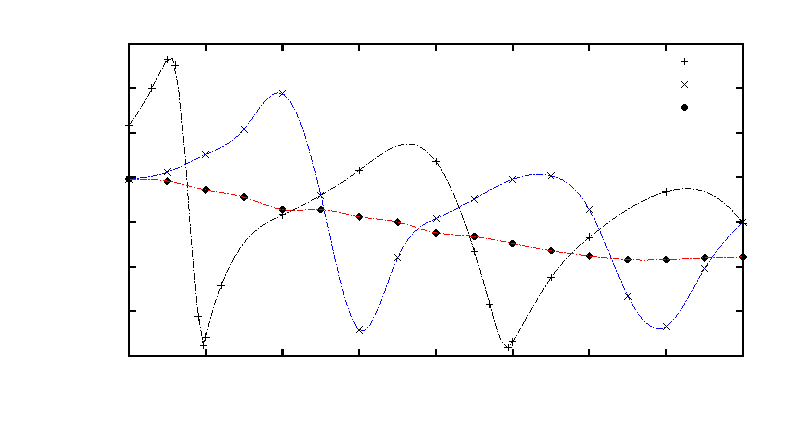
\includegraphics{stichkabel-04}}%
    \gplfronttext
  \end{picture}%
\endgroup

			\caption{\centering Zusammenfassung der gemessenen Übertragungsfunktionen des Koaxialkabels mit verschiedenen Stichkabeln: Peak-to-Peak-Spannung $U_{pp}$ über Frequenz $f$} %fick dich schröter
			\label{diagramm_stichkabel_alles}
		\end{figure}

	% \subsubsection{adrienn-levai} % (fold)
	% \label{ssub:koaxialkabel_mit_eingef_gtem_stichkabel}
	
	
	% 	\begin{figure}[H]
	% 		\center
	% 		
\includegraphics[scale = 0.2]{messwerte/adrienn-levai-nude-sandy-booty-03.jpg}
	% 	\end{figure}

	% subsubsection koaxialkabel_mit_eingef_gtem_stichkabel (end)

	\subsubsection{Koaxialkabel mit doppeltem Stichkabel} % (fold)
	\label{ssub:koaxialkabel_mit_doppeltem_stichkabel}

		Im Folgenden wurden die gleichen Messungen ein zweites Mal durchgeführt.
		Hierbei wurde jedoch ein doppelt so langes Stichkabel verwendet.

		\begin{figure}[H]
			\center
			% GNUPLOT: LaTeX picture with Postscript
\begingroup
  \makeatletter
  \providecommand\color[2][]{%
    \GenericError{(gnuplot) \space\space\space\@spaces}{%
      Package color not loaded in conjunction with
      terminal option `colourtext'%
    }{See the gnuplot documentation for explanation.%
    }{Either use 'blacktext' in gnuplot or load the package
      color.sty in LaTeX.}%
    \renewcommand\color[2][]{}%
  }%
  \providecommand\includegraphics[2][]{%
    \GenericError{(gnuplot) \space\space\space\@spaces}{%
      Package graphicx or graphics not loaded%
    }{See the gnuplot documentation for explanation.%
    }{The gnuplot epslatex terminal needs graphicx.sty or graphics.sty.}%
    \renewcommand\includegraphics[2][]{}%
  }%
  \providecommand\rotatebox[2]{#2}%
  \@ifundefined{ifGPcolor}{%
    \newif\ifGPcolor
    \GPcolorfalse
  }{}%
  \@ifundefined{ifGPblacktext}{%
    \newif\ifGPblacktext
    \GPblacktexttrue
  }{}%
  % define a \g@addto@macro without @ in the name:
  \let\gplgaddtomacro\g@addto@macro
  % define empty templates for all commands taking text:
  \gdef\gplbacktext{}%
  \gdef\gplfronttext{}%
  \makeatother
  \ifGPblacktext
    % no textcolor at all
    \def\colorrgb#1{}%
    \def\colorgray#1{}%
  \else
    % gray or color?
    \ifGPcolor
      \def\colorrgb#1{\color[rgb]{#1}}%
      \def\colorgray#1{\color[gray]{#1}}%
      \expandafter\def\csname LTw\endcsname{\color{white}}%
      \expandafter\def\csname LTb\endcsname{\color{black}}%
      \expandafter\def\csname LTa\endcsname{\color{black}}%
      \expandafter\def\csname LT0\endcsname{\color[rgb]{1,0,0}}%
      \expandafter\def\csname LT1\endcsname{\color[rgb]{0,1,0}}%
      \expandafter\def\csname LT2\endcsname{\color[rgb]{0,0,1}}%
      \expandafter\def\csname LT3\endcsname{\color[rgb]{1,0,1}}%
      \expandafter\def\csname LT4\endcsname{\color[rgb]{0,1,1}}%
      \expandafter\def\csname LT5\endcsname{\color[rgb]{1,1,0}}%
      \expandafter\def\csname LT6\endcsname{\color[rgb]{0,0,0}}%
      \expandafter\def\csname LT7\endcsname{\color[rgb]{1,0.3,0}}%
      \expandafter\def\csname LT8\endcsname{\color[rgb]{0.5,0.5,0.5}}%
    \else
      % gray
      \def\colorrgb#1{\color{black}}%
      \def\colorgray#1{\color[gray]{#1}}%
      \expandafter\def\csname LTw\endcsname{\color{white}}%
      \expandafter\def\csname LTb\endcsname{\color{black}}%
      \expandafter\def\csname LTa\endcsname{\color{black}}%
      \expandafter\def\csname LT0\endcsname{\color{black}}%
      \expandafter\def\csname LT1\endcsname{\color{black}}%
      \expandafter\def\csname LT2\endcsname{\color{black}}%
      \expandafter\def\csname LT3\endcsname{\color{black}}%
      \expandafter\def\csname LT4\endcsname{\color{black}}%
      \expandafter\def\csname LT5\endcsname{\color{black}}%
      \expandafter\def\csname LT6\endcsname{\color{black}}%
      \expandafter\def\csname LT7\endcsname{\color{black}}%
      \expandafter\def\csname LT8\endcsname{\color{black}}%
    \fi
  \fi
  \setlength{\unitlength}{0.0500bp}%
  \begin{picture}(7370.00,3968.00)%
    \gplgaddtomacro\gplbacktext{%
      \csname LTb\endcsname%
      \put(946,704){\makebox(0,0)[r]{\strut{} 0}}%
      \put(946,1132){\makebox(0,0)[r]{\strut{} 50}}%
      \put(946,1561){\makebox(0,0)[r]{\strut{} 100}}%
      \put(946,1989){\makebox(0,0)[r]{\strut{} 150}}%
      \put(946,2418){\makebox(0,0)[r]{\strut{} 200}}%
      \put(946,2846){\makebox(0,0)[r]{\strut{} 250}}%
      \put(946,3275){\makebox(0,0)[r]{\strut{} 300}}%
      \put(946,3703){\makebox(0,0)[r]{\strut{} 350}}%
      \put(1078,484){\makebox(0,0){\strut{} 10}}%
      \put(1815,484){\makebox(0,0){\strut{} 20}}%
      \put(2552,484){\makebox(0,0){\strut{} 30}}%
      \put(3289,484){\makebox(0,0){\strut{} 40}}%
      \put(4026,484){\makebox(0,0){\strut{} 50}}%
      \put(4762,484){\makebox(0,0){\strut{} 60}}%
      \put(5499,484){\makebox(0,0){\strut{} 70}}%
      \put(6236,484){\makebox(0,0){\strut{} 80}}%
      \put(6973,484){\makebox(0,0){\strut{} 90}}%
      \put(176,2203){\rotatebox{-270}{\makebox(0,0){\strut{}$U_{pp}$ \ [mV]}}}%
      \put(4025,154){\makebox(0,0){\strut{}$f$ \ [MHz]}}%
    }%
    \gplgaddtomacro\gplfronttext{%
      \csname LTb\endcsname%
      \put(5986,3530){\makebox(0,0)[r]{\strut{}offen}}%
      \csname LTb\endcsname%
      \put(5986,3310){\makebox(0,0)[r]{\strut{}kurzgeschlossen}}%
      \csname LTb\endcsname%
      \put(5986,3090){\makebox(0,0)[r]{\strut{}angepasst}}%
    }%
    \gplbacktext
    \put(0,0){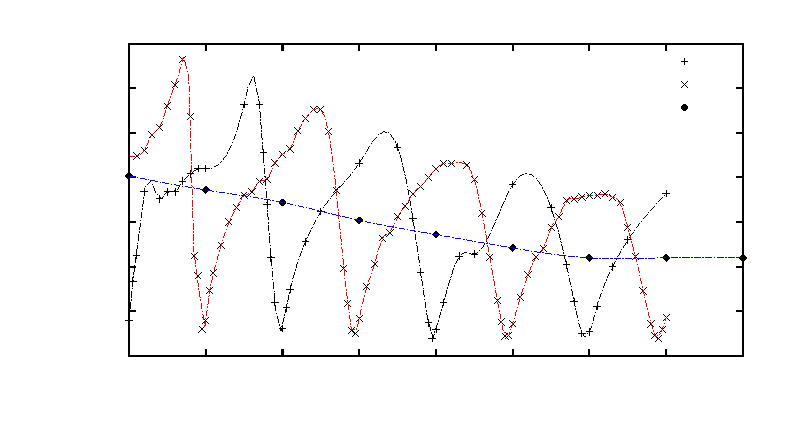
\includegraphics{stichkabel2-04}}%
    \gplfronttext
  \end{picture}%
\endgroup

			\caption{\centering Zusammenfassung der gemessenen Übertragungsfunktionen des Koaxialkabels mit verschiedenen Stichkabeln doppelter Länge: Peak-to-Peak-Spannung $U_{pp}$ über Frequenz $f$} %fick dich schröter
			\label{diagramm_stichkabel2}
		\end{figure}

		Die Theorie besagt, dass sich qualitativ an dem Spannungsverläufen nichts ändern sollte.
		Die Minima entstehen an doppelt so vielen Stellen.
		Die Messung bestätigte dies.
		Aus diesem Grund soll hier nur eine Zusammenfassung der Graphen gezeigt werden. \\

		Aufgrund der letzten beiden Kapitel wurde noch einmal verdeutlicht, dass eine Anpassung der Widerstände im Allgemeinen notwendig ist.
		Allerdings lassen sich ohne Anpassung auch der Verkürzungsfaktor oder der Wellenwiderstand eines Kabels bestimmen.
		Die Regelmäßigkeit von Minima und Maxima lassen sich hier also auch als Vorteil nutzen.
	
	% subsubsection koaxialkabel_mit_doppeltem_stichkabel (end)

	\subsubsection{Verhalten von Rechteckimpulsen} % (fold)
	\label{ssub:verhalten_von_rechteckimpulsen}
	
		Bisher wurden periodische Signale untersucht.
		So konnten sich in den Kabeln stehende Wellen ausbilden und die Übertragungsfunktion abändern.
		Dieses Verhalten gilt im Allgemeinen nicht für Impulse.

		In Abbildung \ref{schaltung_impuls_1} ist die Schaltung, welche folgender Messung zugrunde liegt, angegeben.
		Für diesen Versuchsteil wurde ein Koaxialkabel mit einer Länge von $1$m und ein langes Stichkabel mit einer Länge von $25$m verwendet.
		Ein einzelner Rechteckimpuls erzeugte dann den Graphen in Abbildung \ref{diagramm_impuls_1} auf dem Oszilloskop.

		\begin{figure}[H]
			\center
			% GNUPLOT: LaTeX picture with Postscript
\begingroup
  \makeatletter
  \providecommand\color[2][]{%
    \GenericError{(gnuplot) \space\space\space\@spaces}{%
      Package color not loaded in conjunction with
      terminal option `colourtext'%
    }{See the gnuplot documentation for explanation.%
    }{Either use 'blacktext' in gnuplot or load the package
      color.sty in LaTeX.}%
    \renewcommand\color[2][]{}%
  }%
  \providecommand\includegraphics[2][]{%
    \GenericError{(gnuplot) \space\space\space\@spaces}{%
      Package graphicx or graphics not loaded%
    }{See the gnuplot documentation for explanation.%
    }{The gnuplot epslatex terminal needs graphicx.sty or graphics.sty.}%
    \renewcommand\includegraphics[2][]{}%
  }%
  \providecommand\rotatebox[2]{#2}%
  \@ifundefined{ifGPcolor}{%
    \newif\ifGPcolor
    \GPcolorfalse
  }{}%
  \@ifundefined{ifGPblacktext}{%
    \newif\ifGPblacktext
    \GPblacktexttrue
  }{}%
  % define a \g@addto@macro without @ in the name:
  \let\gplgaddtomacro\g@addto@macro
  % define empty templates for all commands taking text:
  \gdef\gplbacktext{}%
  \gdef\gplfronttext{}%
  \makeatother
  \ifGPblacktext
    % no textcolor at all
    \def\colorrgb#1{}%
    \def\colorgray#1{}%
  \else
    % gray or color?
    \ifGPcolor
      \def\colorrgb#1{\color[rgb]{#1}}%
      \def\colorgray#1{\color[gray]{#1}}%
      \expandafter\def\csname LTw\endcsname{\color{white}}%
      \expandafter\def\csname LTb\endcsname{\color{black}}%
      \expandafter\def\csname LTa\endcsname{\color{black}}%
      \expandafter\def\csname LT0\endcsname{\color[rgb]{1,0,0}}%
      \expandafter\def\csname LT1\endcsname{\color[rgb]{0,1,0}}%
      \expandafter\def\csname LT2\endcsname{\color[rgb]{0,0,1}}%
      \expandafter\def\csname LT3\endcsname{\color[rgb]{1,0,1}}%
      \expandafter\def\csname LT4\endcsname{\color[rgb]{0,1,1}}%
      \expandafter\def\csname LT5\endcsname{\color[rgb]{1,1,0}}%
      \expandafter\def\csname LT6\endcsname{\color[rgb]{0,0,0}}%
      \expandafter\def\csname LT7\endcsname{\color[rgb]{1,0.3,0}}%
      \expandafter\def\csname LT8\endcsname{\color[rgb]{0.5,0.5,0.5}}%
    \else
      % gray
      \def\colorrgb#1{\color{black}}%
      \def\colorgray#1{\color[gray]{#1}}%
      \expandafter\def\csname LTw\endcsname{\color{white}}%
      \expandafter\def\csname LTb\endcsname{\color{black}}%
      \expandafter\def\csname LTa\endcsname{\color{black}}%
      \expandafter\def\csname LT0\endcsname{\color{black}}%
      \expandafter\def\csname LT1\endcsname{\color{black}}%
      \expandafter\def\csname LT2\endcsname{\color{black}}%
      \expandafter\def\csname LT3\endcsname{\color{black}}%
      \expandafter\def\csname LT4\endcsname{\color{black}}%
      \expandafter\def\csname LT5\endcsname{\color{black}}%
      \expandafter\def\csname LT6\endcsname{\color{black}}%
      \expandafter\def\csname LT7\endcsname{\color{black}}%
      \expandafter\def\csname LT8\endcsname{\color{black}}%
    \fi
  \fi
  \setlength{\unitlength}{0.0500bp}%
  \begin{picture}(7370.00,3968.00)%
    \gplgaddtomacro\gplbacktext{%
      \csname LTb\endcsname%
      \put(946,704){\makebox(0,0)[r]{\strut{}-0.7}}%
      \put(946,1037){\makebox(0,0)[r]{\strut{}-0.6}}%
      \put(946,1370){\makebox(0,0)[r]{\strut{}-0.5}}%
      \put(946,1704){\makebox(0,0)[r]{\strut{}-0.4}}%
      \put(946,2037){\makebox(0,0)[r]{\strut{}-0.3}}%
      \put(946,2370){\makebox(0,0)[r]{\strut{}-0.2}}%
      \put(946,2703){\makebox(0,0)[r]{\strut{}-0.1}}%
      \put(946,3037){\makebox(0,0)[r]{\strut{} 0}}%
      \put(946,3370){\makebox(0,0)[r]{\strut{} 0.1}}%
      \put(946,3703){\makebox(0,0)[r]{\strut{} 0.2}}%
      \put(1078,484){\makebox(0,0){\strut{}-2e-07}}%
      \put(1920,484){\makebox(0,0){\strut{} 0}}%
      \put(2762,484){\makebox(0,0){\strut{} 2e-07}}%
      \put(3604,484){\makebox(0,0){\strut{} 4e-07}}%
      \put(4447,484){\makebox(0,0){\strut{} 6e-07}}%
      \put(5289,484){\makebox(0,0){\strut{} 8e-07}}%
      \put(6131,484){\makebox(0,0){\strut{} 1e-06}}%
      \put(6973,484){\makebox(0,0){\strut{} 1.2e-06}}%
      \put(176,2203){\rotatebox{-270}{\makebox(0,0){\strut{}$U$}}}%
      \put(4025,154){\makebox(0,0){\strut{}$t$}}%
    }%
    \gplgaddtomacro\gplfronttext{%
      \csname LTb\endcsname%
      \put(5986,3530){\makebox(0,0)[r]{\strut{}Messwerte}}%
    }%
    \gplbacktext
    \put(0,0){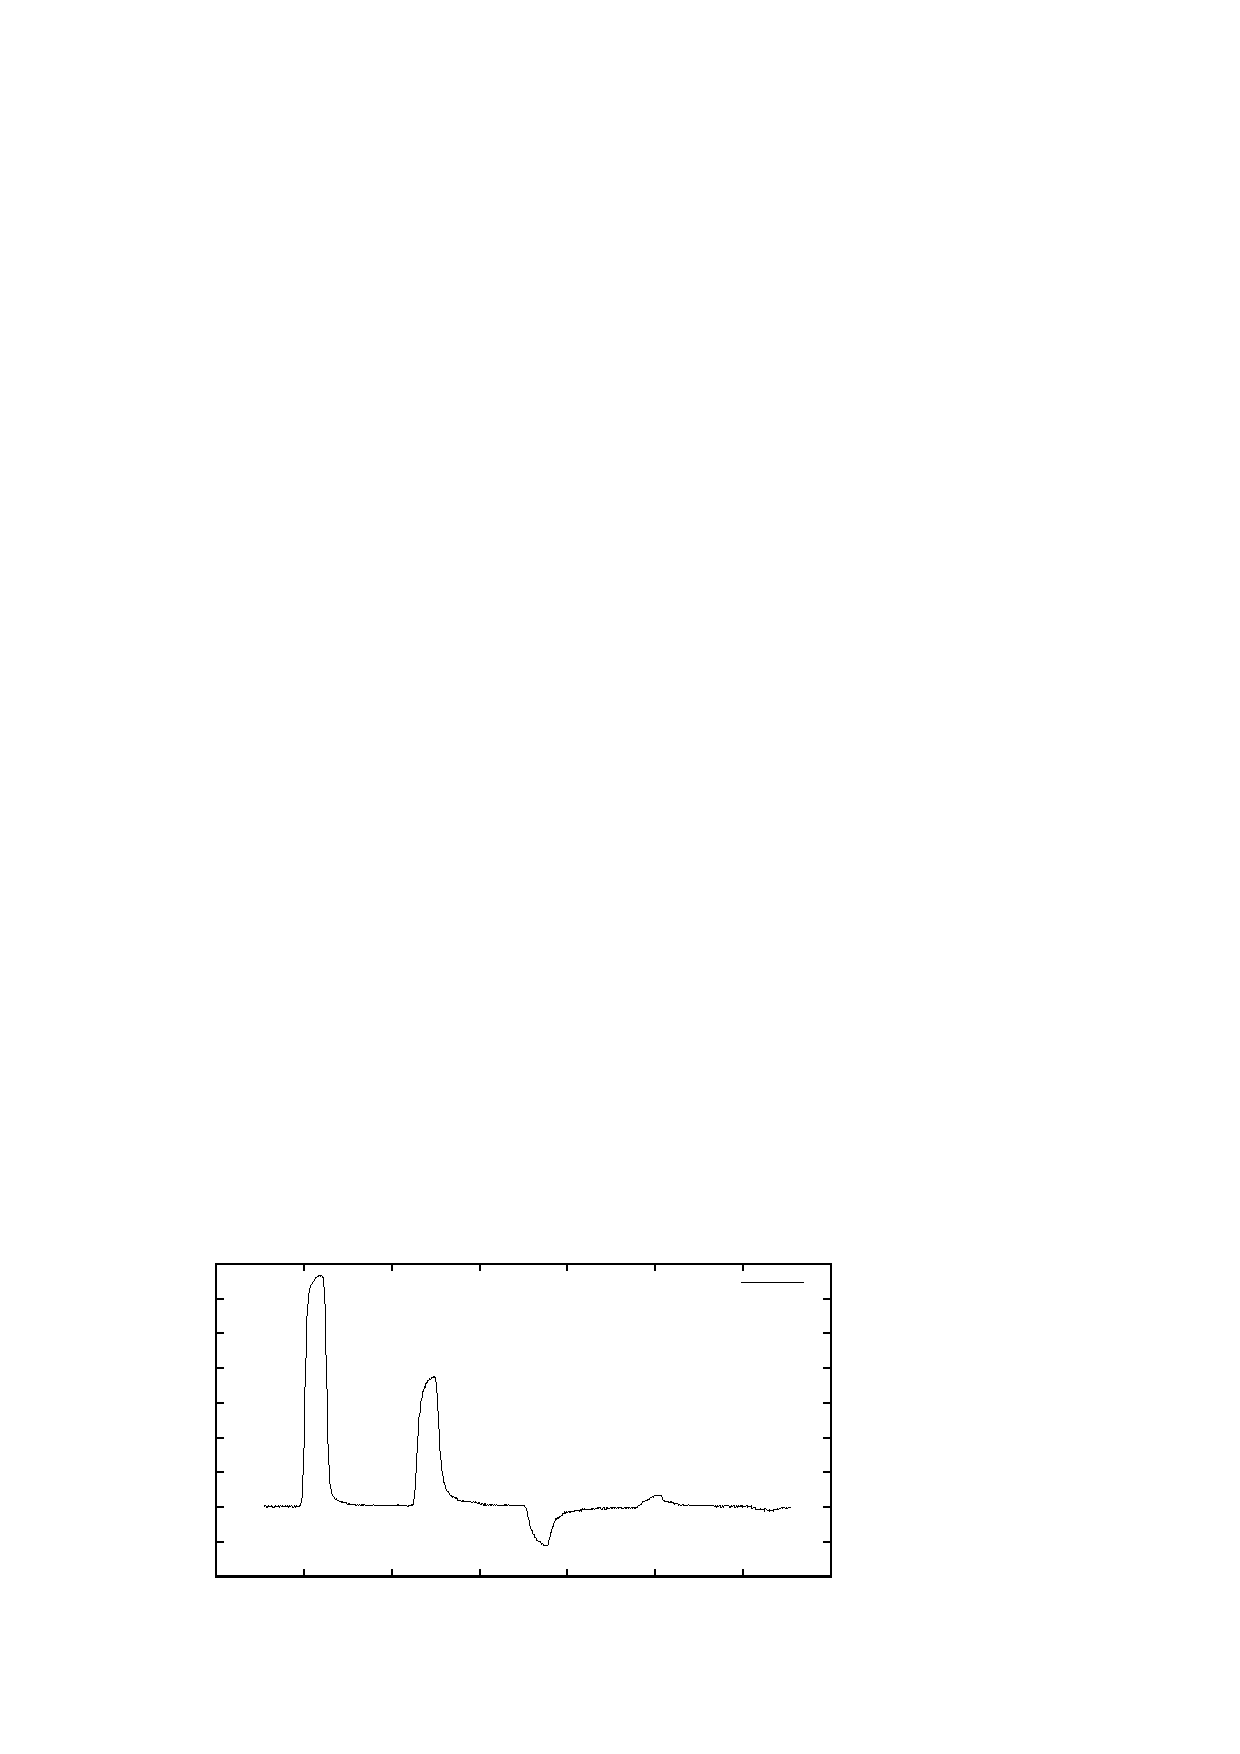
\includegraphics{impuls-offen-01}}%
    \gplfronttext
  \end{picture}%
\endgroup

			\caption{\centering Resultierende Kurve am Oszilloskop durch Senden eines Rechteckimpulses unter Verwendung der Schaltung aus Abbildung \ref{schaltung_impuls_1}: \\ Spannung $U$ über Zeit $t$}
			\label{diagramm_impuls_1}
		\end{figure}

		Der erste sichtbare Impuls ist der vom Impulsgenerator ausgesendete Impuls.
		Wie in den Grundlagen vorhergesagt, wird auch hier am offenen Ende des langen Stichkabels der gesendete Impuls reflektiert, sodass im Graphen mehr als nur dieser zu sehen ist.
		Nach Empfang des gesendeten Impulses im Oszilloskop läuft dieser weiter durch das Stichkabel.
		Aufgrund der vergleichsweise großen Länge des Stichkabels ist hier die Laufzeit des Impulses größer als dessen Breite.
		Am Ende des Stichkabels wird dieser dann am offenen Ende, also ohne Umkehrung der Amplitude, reflektiert und zurückgesendet.
		Auch jetzt muss das Stichkabel wieder bis zum Oszilloskop durchlaufen werden.
		Der zweite Impuls im Diagramm stellt damit die erste Reflexion des gesendeten Impulses dar.
		Nachdem der reflektierte Impuls vom Oszilloskop gemessen wurde, könnte man vermuten, dass er durch den $50\Omega$ Eingangswiderstand absorbiert wird.
		Dies geschieht jedoch nicht, da auch der Impulsgenerator einen Ausgangswiderstand von $50\Omega$ besitzt.
		Dadurch entsteht eine Parallelschaltung von zwei $50\Omega$ Widerständen.
		Der Gesamtwiderstand beträgt also $25\Omega$ und ist damit nicht mehr an den Wellenwiderstand angepasst.
		Insbesondere ist er auch noch kleiner als dieser.
		Es findet also eine Reflexion an einem in einer abgeschwächten Form vorkommenden geschlossenen Ende statt.
		Der zweite reflektierte Impuls kehrt sich also um und fließt wieder durch das Stichkabel.
		Im Stichkabel passiert nun wieder genau das Gleiche wie vorher.
		Der Impuls wird am offenen Ende reflektiert, zurückgesendet und vom Oszilloskop mit einer negativen Amplitude gemessen.
		Nach dieser Messung wiederholt sich dieses Prinzip bis der Impuls im Rauschen untergeht. 
		Da alle Kabel einen geringen ohmschen Widerstand besitzen, muss natürlich auch die Amplitude der Impulse entlang des Kabels abnehmen.

		\begin{figure}[H]
			\center
			% GNUPLOT: LaTeX picture with Postscript
\begingroup
  \makeatletter
  \providecommand\color[2][]{%
    \GenericError{(gnuplot) \space\space\space\@spaces}{%
      Package color not loaded in conjunction with
      terminal option `colourtext'%
    }{See the gnuplot documentation for explanation.%
    }{Either use 'blacktext' in gnuplot or load the package
      color.sty in LaTeX.}%
    \renewcommand\color[2][]{}%
  }%
  \providecommand\includegraphics[2][]{%
    \GenericError{(gnuplot) \space\space\space\@spaces}{%
      Package graphicx or graphics not loaded%
    }{See the gnuplot documentation for explanation.%
    }{The gnuplot epslatex terminal needs graphicx.sty or graphics.sty.}%
    \renewcommand\includegraphics[2][]{}%
  }%
  \providecommand\rotatebox[2]{#2}%
  \@ifundefined{ifGPcolor}{%
    \newif\ifGPcolor
    \GPcolorfalse
  }{}%
  \@ifundefined{ifGPblacktext}{%
    \newif\ifGPblacktext
    \GPblacktexttrue
  }{}%
  % define a \g@addto@macro without @ in the name:
  \let\gplgaddtomacro\g@addto@macro
  % define empty templates for all commands taking text:
  \gdef\gplbacktext{}%
  \gdef\gplfronttext{}%
  \makeatother
  \ifGPblacktext
    % no textcolor at all
    \def\colorrgb#1{}%
    \def\colorgray#1{}%
  \else
    % gray or color?
    \ifGPcolor
      \def\colorrgb#1{\color[rgb]{#1}}%
      \def\colorgray#1{\color[gray]{#1}}%
      \expandafter\def\csname LTw\endcsname{\color{white}}%
      \expandafter\def\csname LTb\endcsname{\color{black}}%
      \expandafter\def\csname LTa\endcsname{\color{black}}%
      \expandafter\def\csname LT0\endcsname{\color[rgb]{1,0,0}}%
      \expandafter\def\csname LT1\endcsname{\color[rgb]{0,1,0}}%
      \expandafter\def\csname LT2\endcsname{\color[rgb]{0,0,1}}%
      \expandafter\def\csname LT3\endcsname{\color[rgb]{1,0,1}}%
      \expandafter\def\csname LT4\endcsname{\color[rgb]{0,1,1}}%
      \expandafter\def\csname LT5\endcsname{\color[rgb]{1,1,0}}%
      \expandafter\def\csname LT6\endcsname{\color[rgb]{0,0,0}}%
      \expandafter\def\csname LT7\endcsname{\color[rgb]{1,0.3,0}}%
      \expandafter\def\csname LT8\endcsname{\color[rgb]{0.5,0.5,0.5}}%
    \else
      % gray
      \def\colorrgb#1{\color{black}}%
      \def\colorgray#1{\color[gray]{#1}}%
      \expandafter\def\csname LTw\endcsname{\color{white}}%
      \expandafter\def\csname LTb\endcsname{\color{black}}%
      \expandafter\def\csname LTa\endcsname{\color{black}}%
      \expandafter\def\csname LT0\endcsname{\color{black}}%
      \expandafter\def\csname LT1\endcsname{\color{black}}%
      \expandafter\def\csname LT2\endcsname{\color{black}}%
      \expandafter\def\csname LT3\endcsname{\color{black}}%
      \expandafter\def\csname LT4\endcsname{\color{black}}%
      \expandafter\def\csname LT5\endcsname{\color{black}}%
      \expandafter\def\csname LT6\endcsname{\color{black}}%
      \expandafter\def\csname LT7\endcsname{\color{black}}%
      \expandafter\def\csname LT8\endcsname{\color{black}}%
    \fi
  \fi
  \setlength{\unitlength}{0.0500bp}%
  \begin{picture}(7370.00,3968.00)%
    \gplgaddtomacro\gplbacktext{%
      \csname LTb\endcsname%
      \put(946,704){\makebox(0,0)[r]{\strut{}-1}}%
      \put(946,1037){\makebox(0,0)[r]{\strut{}-0.8}}%
      \put(946,1370){\makebox(0,0)[r]{\strut{}-0.6}}%
      \put(946,1704){\makebox(0,0)[r]{\strut{}-0.4}}%
      \put(946,2037){\makebox(0,0)[r]{\strut{}-0.2}}%
      \put(946,2370){\makebox(0,0)[r]{\strut{} 0}}%
      \put(946,2703){\makebox(0,0)[r]{\strut{} 0.2}}%
      \put(946,3037){\makebox(0,0)[r]{\strut{} 0.4}}%
      \put(946,3370){\makebox(0,0)[r]{\strut{} 0.6}}%
      \put(946,3703){\makebox(0,0)[r]{\strut{} 0.8}}%
      \put(1078,484){\makebox(0,0){\strut{}-2e-07}}%
      \put(1920,484){\makebox(0,0){\strut{} 0}}%
      \put(2762,484){\makebox(0,0){\strut{} 2e-07}}%
      \put(3604,484){\makebox(0,0){\strut{} 4e-07}}%
      \put(4447,484){\makebox(0,0){\strut{} 6e-07}}%
      \put(5289,484){\makebox(0,0){\strut{} 8e-07}}%
      \put(6131,484){\makebox(0,0){\strut{} 1e-06}}%
      \put(6973,484){\makebox(0,0){\strut{} 1.2e-06}}%
      \put(176,2203){\rotatebox{-270}{\makebox(0,0){\strut{}$U$}}}%
      \put(4025,154){\makebox(0,0){\strut{}$t$}}%
    }%
    \gplgaddtomacro\gplfronttext{%
      \csname LTb\endcsname%
      \put(5986,3530){\makebox(0,0)[r]{\strut{}Channel 1}}%
      \csname LTb\endcsname%
      \put(5986,3310){\makebox(0,0)[r]{\strut{}Channel 2}}%
    }%
    \gplbacktext
    \put(0,0){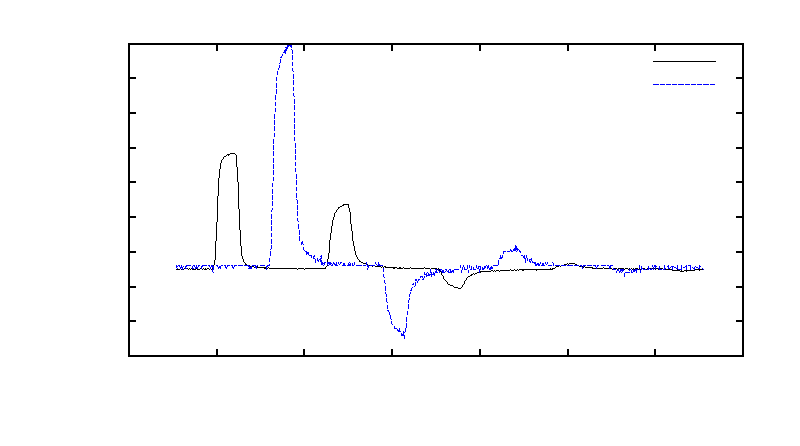
\includegraphics{impuls-offen-02}}%
    \gplfronttext
  \end{picture}%
\endgroup

			\caption{\centering Resultierende Kurven am Oszilloskop durch Senden eines Rechteckimpulses unter Verwendung der Schaltung aus Abbildung \ref{schaltung_impuls_2} mit dem Eingangswiderstand $1$M$\Omega$ für Channel 2: Spannung $U$ über Zeit $t$}
			\label{diagramm_impuls_2}
		\end{figure}

		In Abbildung \ref{diagramm_impuls_2} lässt sich ein analoges Prinzip für die Schaltung aus Abbildung \ref{schaltung_impuls_2} entwerfen, sofern hier der Eingangswiderstand von Channel 2 auf $1$M$\Omega$ gesetzt wird.
		Der Verlauf der Kurve für Channel 1 ist derselbe, wie im vorherigen Versuch.
		Dies liegt daran, dass der hohe Eingangswiderstand an Channel 2 auch als offenes Ende angenähert werden kann.
		Die blaue Kurve stellt dann die Reflexionen am Ende des Stichkabels dar, welche wie oben besprochen, gerade zwischen den bei Channel 1 gemessenen Impulsen entstehen müssen.
		Auch die Amplitudenumkehrungen an den jeweiligen Enden werden hier noch einmal bestätigt. \\

		Die ersten beiden dargestellten Impulse liegen in etwa $2.4\cdot 10^{-7}$s auseinander.
		Der zurücklegte Weg des Impulses zwischen der ersten und der zweiten Messung ist die doppelte Länge des Stichkabels, also $50$m.
		Daraus ergibt sich ebenfalls eine Geschwindigkeit und ein Verkürzungsfaktor.
		\[
			c = \dfrac{\Delta s}{\Delta t} = \dfrac{50\text{m}}{2.4\cdot 10^{-7}\text{s}} \approx 2.08\text{ms}^{-1}
		\]
		\[
			K \approx 0.69
		\]
		Diese Werte stimmen in gewissen Grenzen mit den Vorhergehenden überein und bekräftigen die oben gegebene Erklärung.

		\begin{figure}[H]
			\center
			% % GNUPLOT: LaTeX picture with Postscript
\begingroup
  \makeatletter
  \providecommand\color[2][]{%
    \GenericError{(gnuplot) \space\space\space\@spaces}{%
      Package color not loaded in conjunction with
      terminal option `colourtext'%
    }{See the gnuplot documentation for explanation.%
    }{Either use 'blacktext' in gnuplot or load the package
      color.sty in LaTeX.}%
    \renewcommand\color[2][]{}%
  }%
  \providecommand\includegraphics[2][]{%
    \GenericError{(gnuplot) \space\space\space\@spaces}{%
      Package graphicx or graphics not loaded%
    }{See the gnuplot documentation for explanation.%
    }{The gnuplot epslatex terminal needs graphicx.sty or graphics.sty.}%
    \renewcommand\includegraphics[2][]{}%
  }%
  \providecommand\rotatebox[2]{#2}%
  \@ifundefined{ifGPcolor}{%
    \newif\ifGPcolor
    \GPcolorfalse
  }{}%
  \@ifundefined{ifGPblacktext}{%
    \newif\ifGPblacktext
    \GPblacktexttrue
  }{}%
  % define a \g@addto@macro without @ in the name:
  \let\gplgaddtomacro\g@addto@macro
  % define empty templates for all commands taking text:
  \gdef\gplbacktext{}%
  \gdef\gplfronttext{}%
  \makeatother
  \ifGPblacktext
    % no textcolor at all
    \def\colorrgb#1{}%
    \def\colorgray#1{}%
  \else
    % gray or color?
    \ifGPcolor
      \def\colorrgb#1{\color[rgb]{#1}}%
      \def\colorgray#1{\color[gray]{#1}}%
      \expandafter\def\csname LTw\endcsname{\color{white}}%
      \expandafter\def\csname LTb\endcsname{\color{black}}%
      \expandafter\def\csname LTa\endcsname{\color{black}}%
      \expandafter\def\csname LT0\endcsname{\color[rgb]{1,0,0}}%
      \expandafter\def\csname LT1\endcsname{\color[rgb]{0,1,0}}%
      \expandafter\def\csname LT2\endcsname{\color[rgb]{0,0,1}}%
      \expandafter\def\csname LT3\endcsname{\color[rgb]{1,0,1}}%
      \expandafter\def\csname LT4\endcsname{\color[rgb]{0,1,1}}%
      \expandafter\def\csname LT5\endcsname{\color[rgb]{1,1,0}}%
      \expandafter\def\csname LT6\endcsname{\color[rgb]{0,0,0}}%
      \expandafter\def\csname LT7\endcsname{\color[rgb]{1,0.3,0}}%
      \expandafter\def\csname LT8\endcsname{\color[rgb]{0.5,0.5,0.5}}%
    \else
      % gray
      \def\colorrgb#1{\color{black}}%
      \def\colorgray#1{\color[gray]{#1}}%
      \expandafter\def\csname LTw\endcsname{\color{white}}%
      \expandafter\def\csname LTb\endcsname{\color{black}}%
      \expandafter\def\csname LTa\endcsname{\color{black}}%
      \expandafter\def\csname LT0\endcsname{\color{black}}%
      \expandafter\def\csname LT1\endcsname{\color{black}}%
      \expandafter\def\csname LT2\endcsname{\color{black}}%
      \expandafter\def\csname LT3\endcsname{\color{black}}%
      \expandafter\def\csname LT4\endcsname{\color{black}}%
      \expandafter\def\csname LT5\endcsname{\color{black}}%
      \expandafter\def\csname LT6\endcsname{\color{black}}%
      \expandafter\def\csname LT7\endcsname{\color{black}}%
      \expandafter\def\csname LT8\endcsname{\color{black}}%
    \fi
  \fi
  \setlength{\unitlength}{0.0500bp}%
  \begin{picture}(7370.00,3968.00)%
    \gplgaddtomacro\gplbacktext{%
      \csname LTb\endcsname%
      \put(946,704){\makebox(0,0)[r]{\strut{}-0.7}}%
      \put(946,1037){\makebox(0,0)[r]{\strut{}-0.6}}%
      \put(946,1370){\makebox(0,0)[r]{\strut{}-0.5}}%
      \put(946,1704){\makebox(0,0)[r]{\strut{}-0.4}}%
      \put(946,2037){\makebox(0,0)[r]{\strut{}-0.3}}%
      \put(946,2370){\makebox(0,0)[r]{\strut{}-0.2}}%
      \put(946,2703){\makebox(0,0)[r]{\strut{}-0.1}}%
      \put(946,3037){\makebox(0,0)[r]{\strut{} 0}}%
      \put(946,3370){\makebox(0,0)[r]{\strut{} 0.1}}%
      \put(946,3703){\makebox(0,0)[r]{\strut{} 0.2}}%
      \put(1078,484){\makebox(0,0){\strut{}-2e-07}}%
      \put(1920,484){\makebox(0,0){\strut{} 0}}%
      \put(2762,484){\makebox(0,0){\strut{} 2e-07}}%
      \put(3604,484){\makebox(0,0){\strut{} 4e-07}}%
      \put(4447,484){\makebox(0,0){\strut{} 6e-07}}%
      \put(5289,484){\makebox(0,0){\strut{} 8e-07}}%
      \put(6131,484){\makebox(0,0){\strut{} 1e-06}}%
      \put(6973,484){\makebox(0,0){\strut{} 1.2e-06}}%
      \put(176,2203){\rotatebox{-270}{\makebox(0,0){\strut{}$U$}}}%
      \put(4025,154){\makebox(0,0){\strut{}$t$}}%
    }%
    \gplgaddtomacro\gplfronttext{%
      \csname LTb\endcsname%
      \put(5986,3530){\makebox(0,0)[r]{\strut{}Channel 1}}%
    }%
    \gplbacktext
    \put(0,0){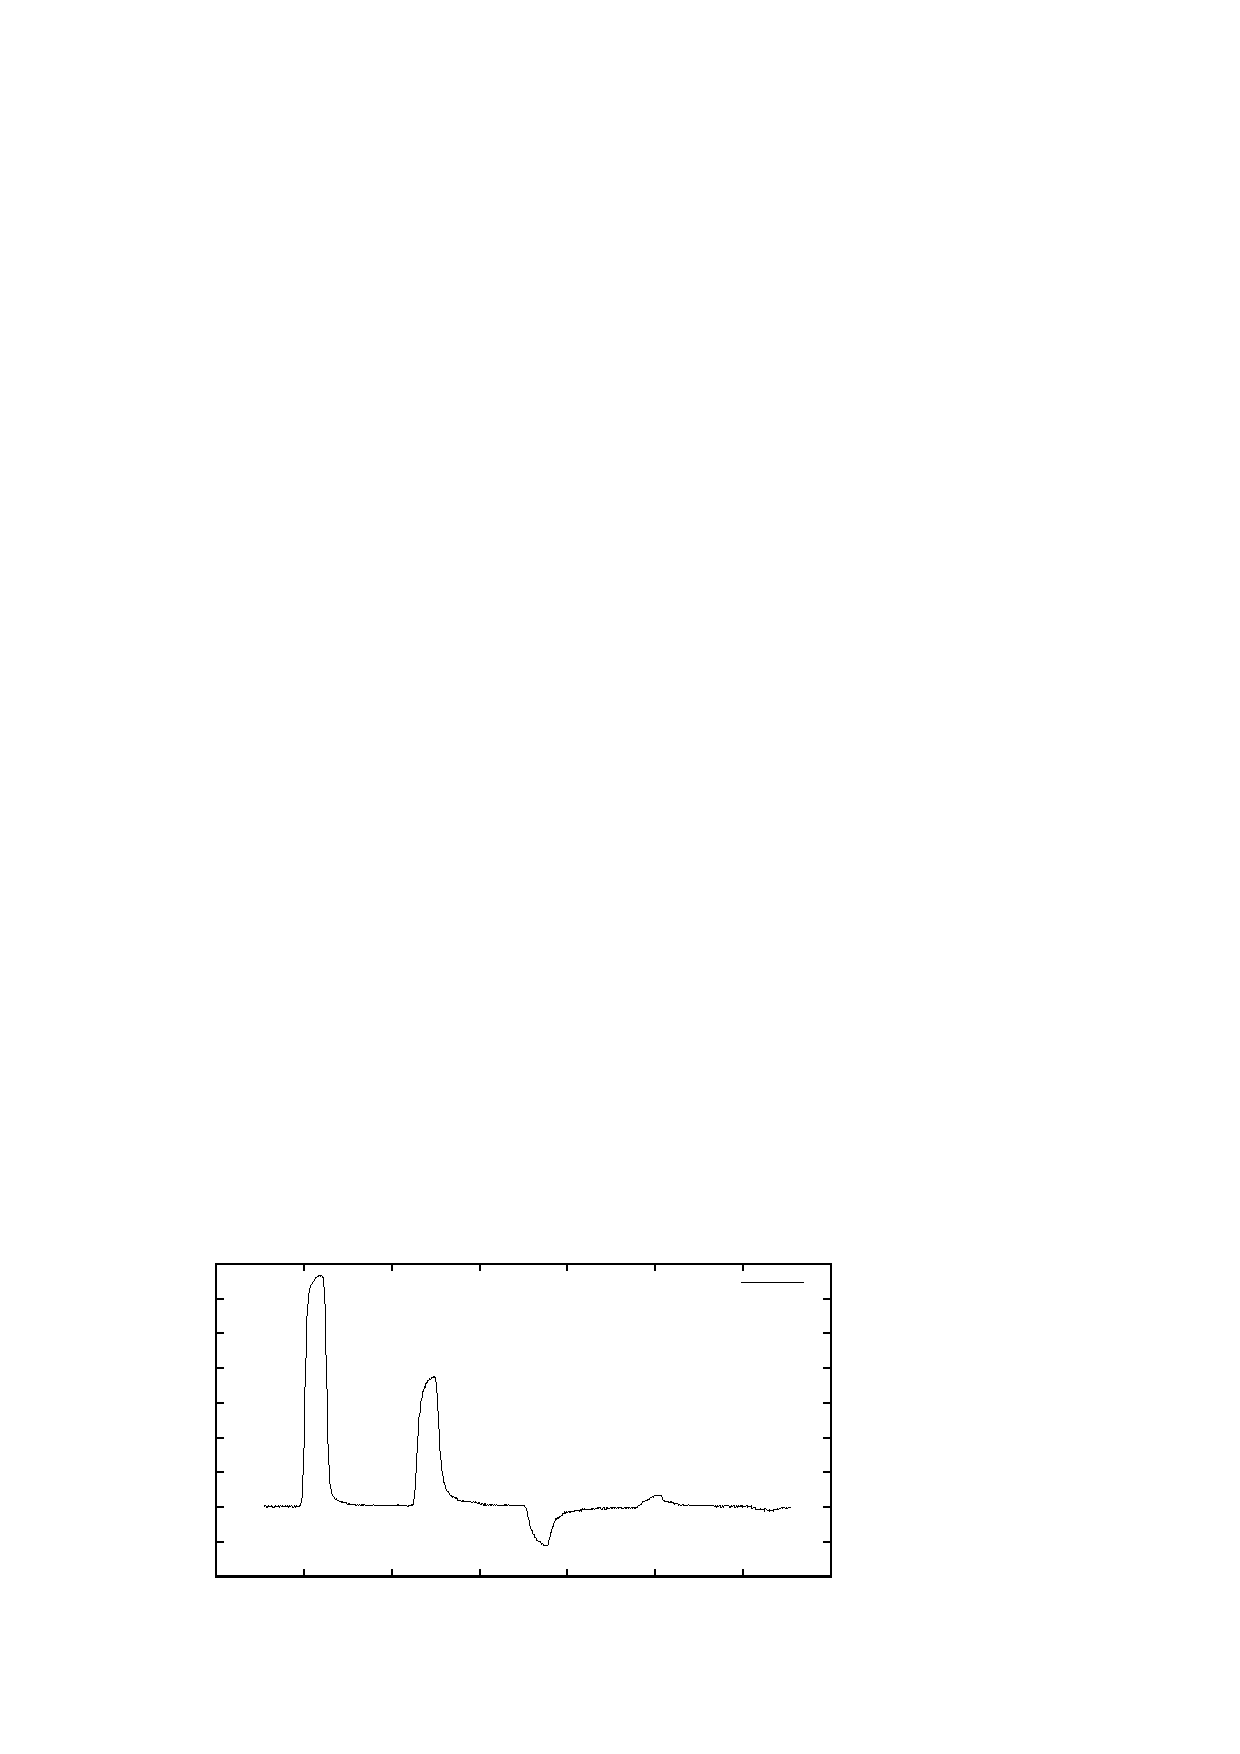
\includegraphics{impuls-offen-03}}%
    \gplfronttext
  \end{picture}%
\endgroup

			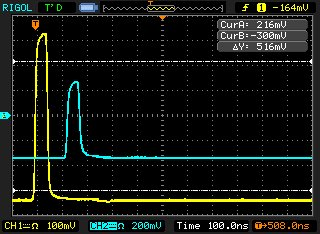
\includegraphics[scale = 0.8]{messwerte/impuls-offen-03.jpg}
			\caption{\centering Resultierende Kurven am Oszilloskop durch Senden eines Rechteckimpulses unter Verwendung der Schaltung aus Abbildung \ref{schaltung_impuls_2} mit dem Eingangswiderstand $50\Omega$ für Channel 2: Spannung $U$ über Zeit $t$}
			\label{diagramm_impuls_3}
		\end{figure}

		Aufgrund der Vollständigkeit wurde in Abbildung \ref{diagramm_impuls_3} noch einmal die Messung des Oszilloskops nach Abänderung des Eingangswiderstands von Channel 2 auf $50\Omega$ gezeigt.
		Hier wurde die Anpassungsbedingung wieder erfüllt.
		Der durch das Stichkabel laufende Impuls wurde hier am Ende des Kabels durch den Eingangswiderstand absorbiert.
		Die Messung bestätigt dies, da keine weiteren reflektierten Impulse im Graph zu sehen sind.

	% subsubsection verhalten_von_rechteckimpulsen (end)

	\subsubsection{Bestimmung des Wellenwiderstandes} % (fold)
	\label{ssub:bestimmung_des_wellenwiderstandes}
	
		Für die Bestimmung des Wellenwiderstandes eines Stichkabels soll das in Kapitel 3 beschriebene Vorgehen realisiert werden.
		Am Ende des Stichkabels wurden drei unterschiedlich genaue Potentiometer befestigt.
		Deren Widerstand wurde in allen Fälle so eingestellt, dass keine Reflexionen mehr sichtbar waren, und dann im Nachhinein gemessen.

		\begin{description}
			\item[$470\Omega$-Poti:]
				\centering $Z_1 = 47.7\Omega$
			\item[$220\Omega$-Poti:]
				$Z_2 = 48.2\Omega$
			\item[$100\Omega$-Poti:]
				$Z_3 = 50.7\Omega$
		\end{description}

		Typische Koaxialkabel, die im Labor und nicht in der TV-Technik verwendet werden, besitzen einen standardisierten Wellenwiderstand von $50\Omega$. \cite{wikikoax}
		Die gemessenen Werte stimmen im Bereich von einigen Ohm mit dem Standard überein.

	% subsubsection bestimmung_des_wellenwiderstandes (end)

% subsection elektromagnetische_wellen_auf_leitungen (end)

\subsection{Modulation und Mischung} % (fold)
\label{sub:modulation_und_mischung}

	Für die Realisierung einer additiven Amplitudenmodulation wurde eine Trägerfrequenz $f_T = 10$MHz und eine Nutzfrequenz von $f_N = 0.1$MHz gewählt.
	Dabei betrugen die Peak-to-Peak-Spannungen $2.28$V für das Trägersignal und $100$mV für Nutzsignal.
	Ein Diagramm des Zeitverlaufs und des Frequenzspektrums werden durch die Abbildungen \ref{diagramm_modulation_amplitude} und \ref{diagramm_modulation_frequenz} gezeigt.
	In guter Näherung weisen beide Graphen den durch die Theorie vorausgesagten Verlauf auf.
	Zu erkennende Abweichungen sind eine gewisse Asymmetrie im Zeitverlauf und zusätzliche periodisch auftauchende Frequenzen im Frequenzspektrum.
	Beide Abweichungen werden durch die Verwendung einer nicht idealen Diode erklärt, deren Kennlinie durch eine gewisse Exponentialfunktion beschrieben werden kann.
	Dieser nicht-lineare Verlauf verursacht das Vorkommen weiterer Frequenzen im Frequenzspektrum.
	Weiterhin wird aber gerade durch diese zusätzlichen Frequenzen der Zeitverlauf des modulierten Signals asymmetrisch.	

	\begin{figure}[H]
		\center
		% GNUPLOT: LaTeX picture with Postscript
\begingroup
  \makeatletter
  \providecommand\color[2][]{%
    \GenericError{(gnuplot) \space\space\space\@spaces}{%
      Package color not loaded in conjunction with
      terminal option `colourtext'%
    }{See the gnuplot documentation for explanation.%
    }{Either use 'blacktext' in gnuplot or load the package
      color.sty in LaTeX.}%
    \renewcommand\color[2][]{}%
  }%
  \providecommand\includegraphics[2][]{%
    \GenericError{(gnuplot) \space\space\space\@spaces}{%
      Package graphicx or graphics not loaded%
    }{See the gnuplot documentation for explanation.%
    }{The gnuplot epslatex terminal needs graphicx.sty or graphics.sty.}%
    \renewcommand\includegraphics[2][]{}%
  }%
  \providecommand\rotatebox[2]{#2}%
  \@ifundefined{ifGPcolor}{%
    \newif\ifGPcolor
    \GPcolorfalse
  }{}%
  \@ifundefined{ifGPblacktext}{%
    \newif\ifGPblacktext
    \GPblacktexttrue
  }{}%
  % define a \g@addto@macro without @ in the name:
  \let\gplgaddtomacro\g@addto@macro
  % define empty templates for all commands taking text:
  \gdef\gplbacktext{}%
  \gdef\gplfronttext{}%
  \makeatother
  \ifGPblacktext
    % no textcolor at all
    \def\colorrgb#1{}%
    \def\colorgray#1{}%
  \else
    % gray or color?
    \ifGPcolor
      \def\colorrgb#1{\color[rgb]{#1}}%
      \def\colorgray#1{\color[gray]{#1}}%
      \expandafter\def\csname LTw\endcsname{\color{white}}%
      \expandafter\def\csname LTb\endcsname{\color{black}}%
      \expandafter\def\csname LTa\endcsname{\color{black}}%
      \expandafter\def\csname LT0\endcsname{\color[rgb]{1,0,0}}%
      \expandafter\def\csname LT1\endcsname{\color[rgb]{0,1,0}}%
      \expandafter\def\csname LT2\endcsname{\color[rgb]{0,0,1}}%
      \expandafter\def\csname LT3\endcsname{\color[rgb]{1,0,1}}%
      \expandafter\def\csname LT4\endcsname{\color[rgb]{0,1,1}}%
      \expandafter\def\csname LT5\endcsname{\color[rgb]{1,1,0}}%
      \expandafter\def\csname LT6\endcsname{\color[rgb]{0,0,0}}%
      \expandafter\def\csname LT7\endcsname{\color[rgb]{1,0.3,0}}%
      \expandafter\def\csname LT8\endcsname{\color[rgb]{0.5,0.5,0.5}}%
    \else
      % gray
      \def\colorrgb#1{\color{black}}%
      \def\colorgray#1{\color[gray]{#1}}%
      \expandafter\def\csname LTw\endcsname{\color{white}}%
      \expandafter\def\csname LTb\endcsname{\color{black}}%
      \expandafter\def\csname LTa\endcsname{\color{black}}%
      \expandafter\def\csname LT0\endcsname{\color{black}}%
      \expandafter\def\csname LT1\endcsname{\color{black}}%
      \expandafter\def\csname LT2\endcsname{\color{black}}%
      \expandafter\def\csname LT3\endcsname{\color{black}}%
      \expandafter\def\csname LT4\endcsname{\color{black}}%
      \expandafter\def\csname LT5\endcsname{\color{black}}%
      \expandafter\def\csname LT6\endcsname{\color{black}}%
      \expandafter\def\csname LT7\endcsname{\color{black}}%
      \expandafter\def\csname LT8\endcsname{\color{black}}%
    \fi
  \fi
  \setlength{\unitlength}{0.0500bp}%
  \begin{picture}(7370.00,3968.00)%
    \gplgaddtomacro\gplbacktext{%
      \csname LTb\endcsname%
      \put(1078,704){\makebox(0,0)[r]{\strut{}-0.04}}%
      \put(1078,1204){\makebox(0,0)[r]{\strut{}-0.02}}%
      \put(1078,1704){\makebox(0,0)[r]{\strut{} 0}}%
      \put(1078,2204){\makebox(0,0)[r]{\strut{} 0.02}}%
      \put(1078,2703){\makebox(0,0)[r]{\strut{} 0.04}}%
      \put(1078,3203){\makebox(0,0)[r]{\strut{} 0.06}}%
      \put(1078,3703){\makebox(0,0)[r]{\strut{} 0.08}}%
      \put(1210,484){\makebox(0,0){\strut{}-1e-05}}%
      \put(2651,484){\makebox(0,0){\strut{}-5e-06}}%
      \put(4092,484){\makebox(0,0){\strut{} 0}}%
      \put(5532,484){\makebox(0,0){\strut{} 5e-06}}%
      \put(6973,484){\makebox(0,0){\strut{} 1e-05}}%
      \put(176,2203){\rotatebox{-270}{\makebox(0,0){\strut{}$U$}}}%
      \put(4091,154){\makebox(0,0){\strut{}$t$ \ [s]}}%
    }%
    \gplgaddtomacro\gplfronttext{%
      \csname LTb\endcsname%
      \put(5986,3530){\makebox(0,0)[r]{\strut{}Messwerte}}%
    }%
    \gplbacktext
    \put(0,0){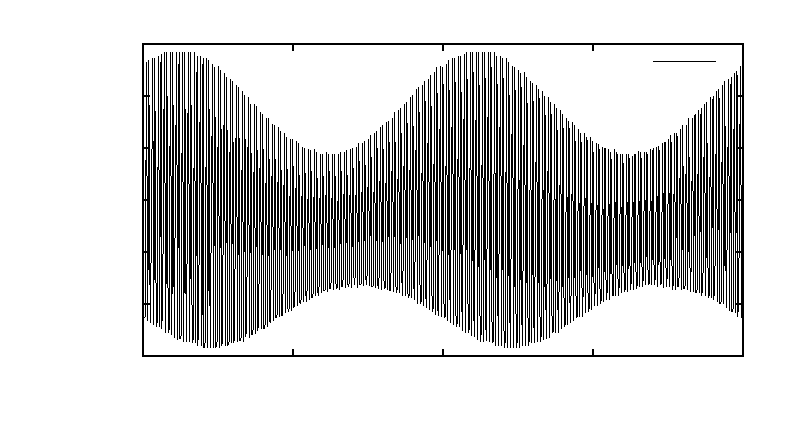
\includegraphics{modulation-amp}}%
    \gplfronttext
  \end{picture}%
\endgroup

		\caption{\centering Zeitverlauf einer additiven Amplitudenmodulation für die angegebenen Frequenzen im Text unter Verwendung der Schaltung aus Abbildung \ref{schaltung_modulation_1}: Spannung $U$ über Zeit $t$}
		\label{diagramm_modulation_amplitude}
	\end{figure}

	\begin{figure}[H]
		\center
		% GNUPLOT: LaTeX picture with Postscript
\begingroup
  \makeatletter
  \providecommand\color[2][]{%
    \GenericError{(gnuplot) \space\space\space\@spaces}{%
      Package color not loaded in conjunction with
      terminal option `colourtext'%
    }{See the gnuplot documentation for explanation.%
    }{Either use 'blacktext' in gnuplot or load the package
      color.sty in LaTeX.}%
    \renewcommand\color[2][]{}%
  }%
  \providecommand\includegraphics[2][]{%
    \GenericError{(gnuplot) \space\space\space\@spaces}{%
      Package graphicx or graphics not loaded%
    }{See the gnuplot documentation for explanation.%
    }{The gnuplot epslatex terminal needs graphicx.sty or graphics.sty.}%
    \renewcommand\includegraphics[2][]{}%
  }%
  \providecommand\rotatebox[2]{#2}%
  \@ifundefined{ifGPcolor}{%
    \newif\ifGPcolor
    \GPcolorfalse
  }{}%
  \@ifundefined{ifGPblacktext}{%
    \newif\ifGPblacktext
    \GPblacktexttrue
  }{}%
  % define a \g@addto@macro without @ in the name:
  \let\gplgaddtomacro\g@addto@macro
  % define empty templates for all commands taking text:
  \gdef\gplbacktext{}%
  \gdef\gplfronttext{}%
  \makeatother
  \ifGPblacktext
    % no textcolor at all
    \def\colorrgb#1{}%
    \def\colorgray#1{}%
  \else
    % gray or color?
    \ifGPcolor
      \def\colorrgb#1{\color[rgb]{#1}}%
      \def\colorgray#1{\color[gray]{#1}}%
      \expandafter\def\csname LTw\endcsname{\color{white}}%
      \expandafter\def\csname LTb\endcsname{\color{black}}%
      \expandafter\def\csname LTa\endcsname{\color{black}}%
      \expandafter\def\csname LT0\endcsname{\color[rgb]{1,0,0}}%
      \expandafter\def\csname LT1\endcsname{\color[rgb]{0,1,0}}%
      \expandafter\def\csname LT2\endcsname{\color[rgb]{0,0,1}}%
      \expandafter\def\csname LT3\endcsname{\color[rgb]{1,0,1}}%
      \expandafter\def\csname LT4\endcsname{\color[rgb]{0,1,1}}%
      \expandafter\def\csname LT5\endcsname{\color[rgb]{1,1,0}}%
      \expandafter\def\csname LT6\endcsname{\color[rgb]{0,0,0}}%
      \expandafter\def\csname LT7\endcsname{\color[rgb]{1,0.3,0}}%
      \expandafter\def\csname LT8\endcsname{\color[rgb]{0.5,0.5,0.5}}%
    \else
      % gray
      \def\colorrgb#1{\color{black}}%
      \def\colorgray#1{\color[gray]{#1}}%
      \expandafter\def\csname LTw\endcsname{\color{white}}%
      \expandafter\def\csname LTb\endcsname{\color{black}}%
      \expandafter\def\csname LTa\endcsname{\color{black}}%
      \expandafter\def\csname LT0\endcsname{\color{black}}%
      \expandafter\def\csname LT1\endcsname{\color{black}}%
      \expandafter\def\csname LT2\endcsname{\color{black}}%
      \expandafter\def\csname LT3\endcsname{\color{black}}%
      \expandafter\def\csname LT4\endcsname{\color{black}}%
      \expandafter\def\csname LT5\endcsname{\color{black}}%
      \expandafter\def\csname LT6\endcsname{\color{black}}%
      \expandafter\def\csname LT7\endcsname{\color{black}}%
      \expandafter\def\csname LT8\endcsname{\color{black}}%
    \fi
  \fi
  \setlength{\unitlength}{0.0500bp}%
  \begin{picture}(7370.00,3968.00)%
    \gplgaddtomacro\gplbacktext{%
      \csname LTb\endcsname%
      \put(594,704){\makebox(0,0)[r]{\strut{} 0}}%
      \put(594,1037){\makebox(0,0)[r]{\strut{} 10}}%
      \put(594,1370){\makebox(0,0)[r]{\strut{} 20}}%
      \put(594,1704){\makebox(0,0)[r]{\strut{} 30}}%
      \put(594,2037){\makebox(0,0)[r]{\strut{} 40}}%
      \put(594,2370){\makebox(0,0)[r]{\strut{} 50}}%
      \put(594,2703){\makebox(0,0)[r]{\strut{} 60}}%
      \put(594,3037){\makebox(0,0)[r]{\strut{} 70}}%
      \put(594,3370){\makebox(0,0)[r]{\strut{} 80}}%
      \put(594,3703){\makebox(0,0)[r]{\strut{} 90}}%
      \put(726,484){\makebox(0,0){\strut{} 9.6}}%
      \put(1507,484){\makebox(0,0){\strut{} 9.7}}%
      \put(2288,484){\makebox(0,0){\strut{} 9.8}}%
      \put(3069,484){\makebox(0,0){\strut{} 9.9}}%
      \put(3849,484){\makebox(0,0){\strut{} 10}}%
      \put(4630,484){\makebox(0,0){\strut{} 10.1}}%
      \put(5411,484){\makebox(0,0){\strut{} 10.2}}%
      \put(6192,484){\makebox(0,0){\strut{} 10.3}}%
      \put(6973,484){\makebox(0,0){\strut{} 10.4}}%
      \put(3849,154){\makebox(0,0){\strut{}$f$ \ [MHz]}}%
    }%
    \gplgaddtomacro\gplfronttext{%
      \csname LTb\endcsname%
      \put(5986,3530){\makebox(0,0)[r]{\strut{}Messwerte}}%
    }%
    \gplbacktext
    \put(0,0){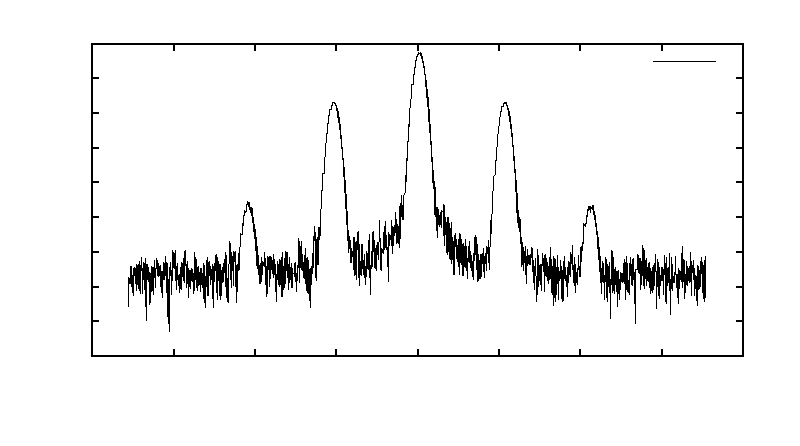
\includegraphics{modulation-freq}}%
    \gplfronttext
  \end{picture}%
\endgroup

		\caption{\centering Frequenzspektrum einer additiven Amplitudenmodulation für die angegebenen Frequenzen im Text unter Verwendung der Schaltung aus Abbildung \ref{schaltung_modulation_1}: Spannung $U$ über Zeit $t$}
		\label{diagramm_modulation_frequenz}
	\end{figure}

% subsection modulation_und_mischung (end)

\subsection{Elektromagnetische Wellen im freien Raum} % (fold)
\label{sub:elektromagnetische_wellen_im_freien_raum}

	\subsubsection{Frequenzanpassung für eine $\lambda/2$-Antenne} % (fold)
	\label{ssub:frequenzanpassung_f_r_eine_}
	
		Eine Frequenzanpassung an die jeweilige Antenne ist notwendig, um im nachfolgenden Versuchsteil eine gute Übertragungsleistung der Signale zu erzielen.
		Sie wurde hier für verschiedene Längen durchgeführt, sodass für die verwendete Längen die Frequenzen direkt abgelesen werden konnten.
		Die Zusammenstellung ist in Abbildung \ref{diagramm_antenne_1} zu sehen.

		\begin{figure}[H]
			\center
			% GNUPLOT: LaTeX picture with Postscript
\begingroup
  \makeatletter
  \providecommand\color[2][]{%
    \GenericError{(gnuplot) \space\space\space\@spaces}{%
      Package color not loaded in conjunction with
      terminal option `colourtext'%
    }{See the gnuplot documentation for explanation.%
    }{Either use 'blacktext' in gnuplot or load the package
      color.sty in LaTeX.}%
    \renewcommand\color[2][]{}%
  }%
  \providecommand\includegraphics[2][]{%
    \GenericError{(gnuplot) \space\space\space\@spaces}{%
      Package graphicx or graphics not loaded%
    }{See the gnuplot documentation for explanation.%
    }{The gnuplot epslatex terminal needs graphicx.sty or graphics.sty.}%
    \renewcommand\includegraphics[2][]{}%
  }%
  \providecommand\rotatebox[2]{#2}%
  \@ifundefined{ifGPcolor}{%
    \newif\ifGPcolor
    \GPcolorfalse
  }{}%
  \@ifundefined{ifGPblacktext}{%
    \newif\ifGPblacktext
    \GPblacktexttrue
  }{}%
  % define a \g@addto@macro without @ in the name:
  \let\gplgaddtomacro\g@addto@macro
  % define empty templates for all commands taking text:
  \gdef\gplbacktext{}%
  \gdef\gplfronttext{}%
  \makeatother
  \ifGPblacktext
    % no textcolor at all
    \def\colorrgb#1{}%
    \def\colorgray#1{}%
  \else
    % gray or color?
    \ifGPcolor
      \def\colorrgb#1{\color[rgb]{#1}}%
      \def\colorgray#1{\color[gray]{#1}}%
      \expandafter\def\csname LTw\endcsname{\color{white}}%
      \expandafter\def\csname LTb\endcsname{\color{black}}%
      \expandafter\def\csname LTa\endcsname{\color{black}}%
      \expandafter\def\csname LT0\endcsname{\color[rgb]{1,0,0}}%
      \expandafter\def\csname LT1\endcsname{\color[rgb]{0,1,0}}%
      \expandafter\def\csname LT2\endcsname{\color[rgb]{0,0,1}}%
      \expandafter\def\csname LT3\endcsname{\color[rgb]{1,0,1}}%
      \expandafter\def\csname LT4\endcsname{\color[rgb]{0,1,1}}%
      \expandafter\def\csname LT5\endcsname{\color[rgb]{1,1,0}}%
      \expandafter\def\csname LT6\endcsname{\color[rgb]{0,0,0}}%
      \expandafter\def\csname LT7\endcsname{\color[rgb]{1,0.3,0}}%
      \expandafter\def\csname LT8\endcsname{\color[rgb]{0.5,0.5,0.5}}%
    \else
      % gray
      \def\colorrgb#1{\color{black}}%
      \def\colorgray#1{\color[gray]{#1}}%
      \expandafter\def\csname LTw\endcsname{\color{white}}%
      \expandafter\def\csname LTb\endcsname{\color{black}}%
      \expandafter\def\csname LTa\endcsname{\color{black}}%
      \expandafter\def\csname LT0\endcsname{\color{black}}%
      \expandafter\def\csname LT1\endcsname{\color{black}}%
      \expandafter\def\csname LT2\endcsname{\color{black}}%
      \expandafter\def\csname LT3\endcsname{\color{black}}%
      \expandafter\def\csname LT4\endcsname{\color{black}}%
      \expandafter\def\csname LT5\endcsname{\color{black}}%
      \expandafter\def\csname LT6\endcsname{\color{black}}%
      \expandafter\def\csname LT7\endcsname{\color{black}}%
      \expandafter\def\csname LT8\endcsname{\color{black}}%
    \fi
  \fi
  \setlength{\unitlength}{0.0500bp}%
  \begin{picture}(7370.00,3968.00)%
    \gplgaddtomacro\gplbacktext{%
      \csname LTb\endcsname%
      \put(946,704){\makebox(0,0)[r]{\strut{} 150}}%
      \put(946,1204){\makebox(0,0)[r]{\strut{} 200}}%
      \put(946,1704){\makebox(0,0)[r]{\strut{} 250}}%
      \put(946,2204){\makebox(0,0)[r]{\strut{} 300}}%
      \put(946,2703){\makebox(0,0)[r]{\strut{} 350}}%
      \put(946,3203){\makebox(0,0)[r]{\strut{} 400}}%
      \put(946,3703){\makebox(0,0)[r]{\strut{} 450}}%
      \put(1078,484){\makebox(0,0){\strut{} 30}}%
      \put(2061,484){\makebox(0,0){\strut{} 40}}%
      \put(3043,484){\makebox(0,0){\strut{} 50}}%
      \put(4026,484){\makebox(0,0){\strut{} 60}}%
      \put(5008,484){\makebox(0,0){\strut{} 70}}%
      \put(5991,484){\makebox(0,0){\strut{} 80}}%
      \put(6973,484){\makebox(0,0){\strut{} 90}}%
      \put(176,2203){\rotatebox{-270}{\makebox(0,0){\strut{}$f$ \ [MHz]}}}%
      \put(4025,154){\makebox(0,0){\strut{}$L$ \ [cm]}}%
    }%
    \gplgaddtomacro\gplfronttext{%
      \csname LTb\endcsname%
      \put(5986,3530){\makebox(0,0)[r]{\strut{}Messwerte}}%
    }%
    \gplbacktext
    \put(0,0){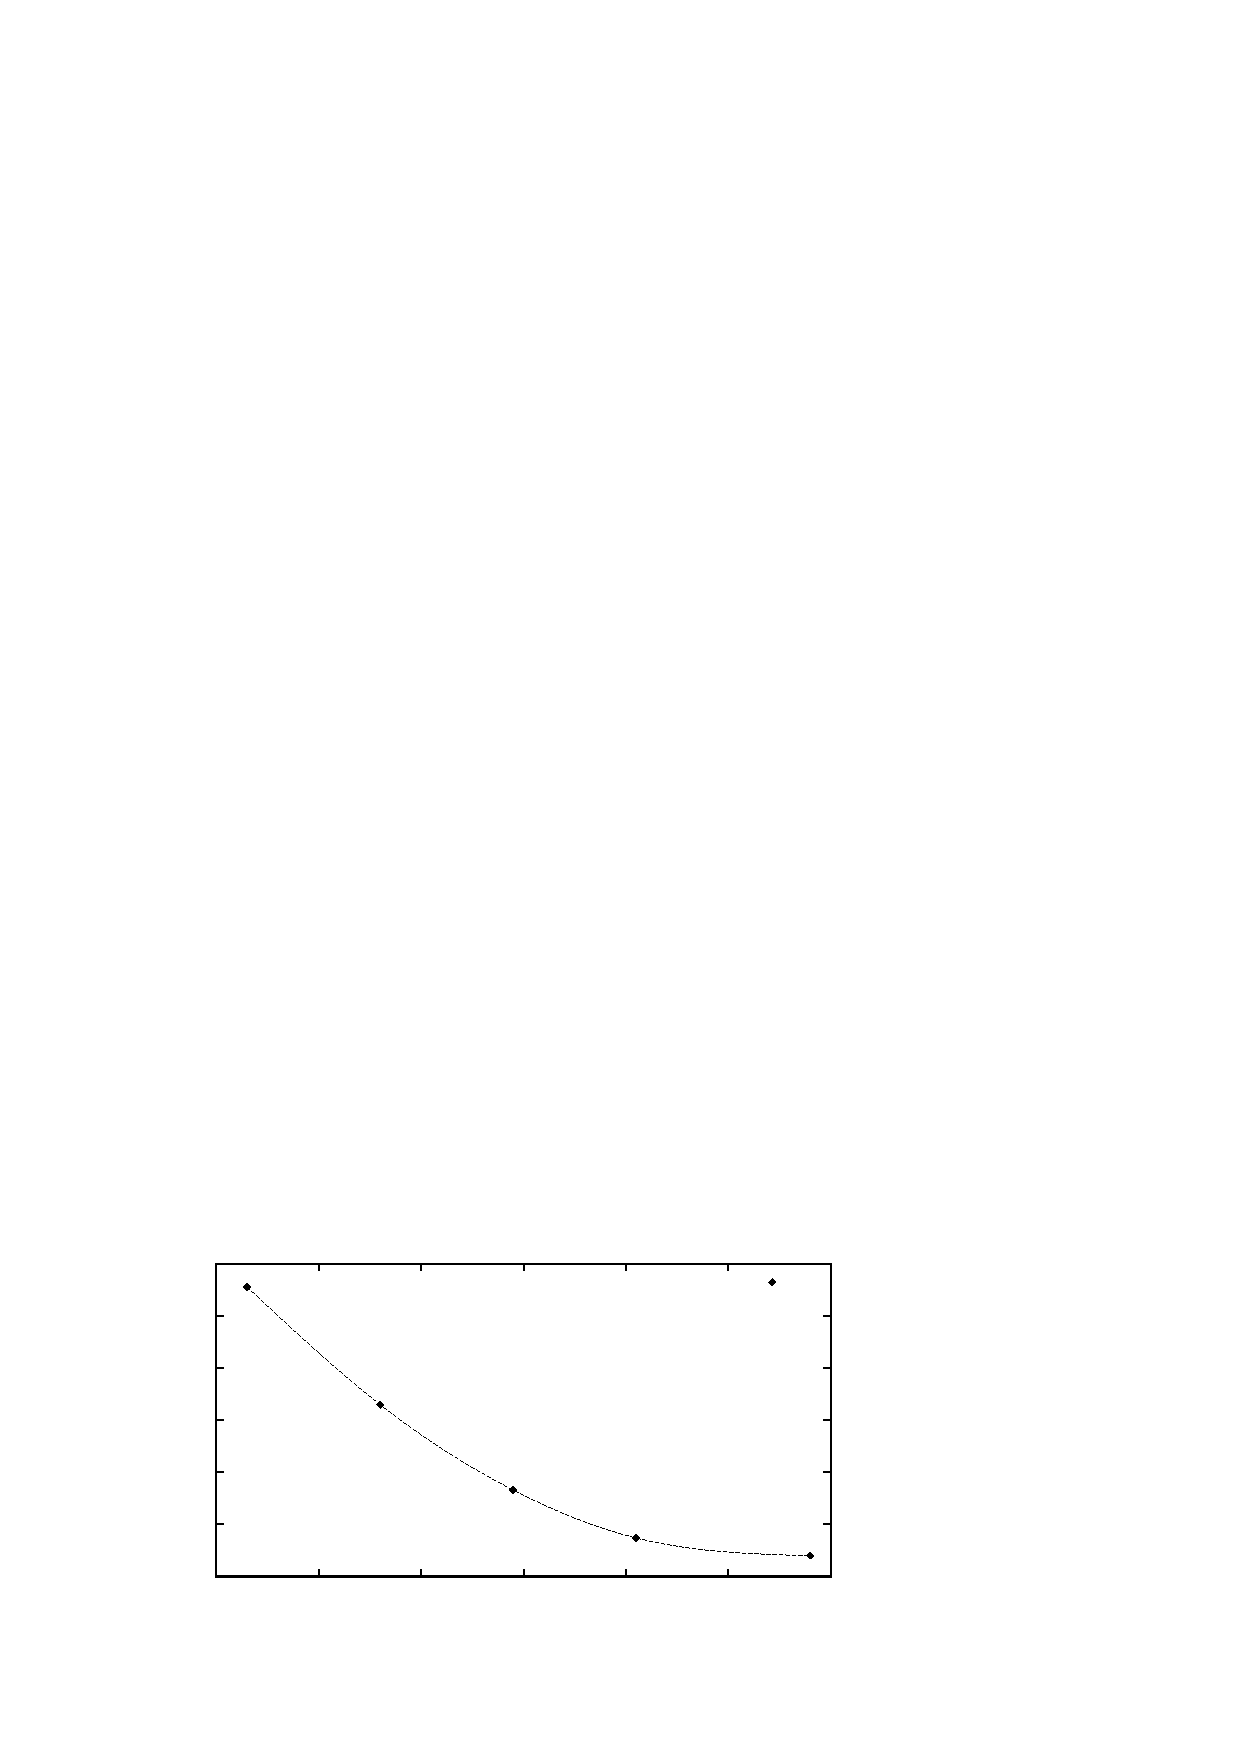
\includegraphics{antenne-01}}%
    \gplfronttext
  \end{picture}%
\endgroup

			\caption{\centering gemessene angepasste Frequenz $f$ in Abhängigkeit der Gesamtlänge $L$ einer $\lambda/2$-Antenne unter Verwendung der Schaltung aus Abbildung \ref{schaltung_antennen_1}}
			\label{diagramm_antenne_1}
		\end{figure}

		\begin{figure}[H]
			\center
			% GNUPLOT: LaTeX picture with Postscript
\begingroup
  \makeatletter
  \providecommand\color[2][]{%
    \GenericError{(gnuplot) \space\space\space\@spaces}{%
      Package color not loaded in conjunction with
      terminal option `colourtext'%
    }{See the gnuplot documentation for explanation.%
    }{Either use 'blacktext' in gnuplot or load the package
      color.sty in LaTeX.}%
    \renewcommand\color[2][]{}%
  }%
  \providecommand\includegraphics[2][]{%
    \GenericError{(gnuplot) \space\space\space\@spaces}{%
      Package graphicx or graphics not loaded%
    }{See the gnuplot documentation for explanation.%
    }{The gnuplot epslatex terminal needs graphicx.sty or graphics.sty.}%
    \renewcommand\includegraphics[2][]{}%
  }%
  \providecommand\rotatebox[2]{#2}%
  \@ifundefined{ifGPcolor}{%
    \newif\ifGPcolor
    \GPcolorfalse
  }{}%
  \@ifundefined{ifGPblacktext}{%
    \newif\ifGPblacktext
    \GPblacktexttrue
  }{}%
  % define a \g@addto@macro without @ in the name:
  \let\gplgaddtomacro\g@addto@macro
  % define empty templates for all commands taking text:
  \gdef\gplbacktext{}%
  \gdef\gplfronttext{}%
  \makeatother
  \ifGPblacktext
    % no textcolor at all
    \def\colorrgb#1{}%
    \def\colorgray#1{}%
  \else
    % gray or color?
    \ifGPcolor
      \def\colorrgb#1{\color[rgb]{#1}}%
      \def\colorgray#1{\color[gray]{#1}}%
      \expandafter\def\csname LTw\endcsname{\color{white}}%
      \expandafter\def\csname LTb\endcsname{\color{black}}%
      \expandafter\def\csname LTa\endcsname{\color{black}}%
      \expandafter\def\csname LT0\endcsname{\color[rgb]{1,0,0}}%
      \expandafter\def\csname LT1\endcsname{\color[rgb]{0,1,0}}%
      \expandafter\def\csname LT2\endcsname{\color[rgb]{0,0,1}}%
      \expandafter\def\csname LT3\endcsname{\color[rgb]{1,0,1}}%
      \expandafter\def\csname LT4\endcsname{\color[rgb]{0,1,1}}%
      \expandafter\def\csname LT5\endcsname{\color[rgb]{1,1,0}}%
      \expandafter\def\csname LT6\endcsname{\color[rgb]{0,0,0}}%
      \expandafter\def\csname LT7\endcsname{\color[rgb]{1,0.3,0}}%
      \expandafter\def\csname LT8\endcsname{\color[rgb]{0.5,0.5,0.5}}%
    \else
      % gray
      \def\colorrgb#1{\color{black}}%
      \def\colorgray#1{\color[gray]{#1}}%
      \expandafter\def\csname LTw\endcsname{\color{white}}%
      \expandafter\def\csname LTb\endcsname{\color{black}}%
      \expandafter\def\csname LTa\endcsname{\color{black}}%
      \expandafter\def\csname LT0\endcsname{\color{black}}%
      \expandafter\def\csname LT1\endcsname{\color{black}}%
      \expandafter\def\csname LT2\endcsname{\color{black}}%
      \expandafter\def\csname LT3\endcsname{\color{black}}%
      \expandafter\def\csname LT4\endcsname{\color{black}}%
      \expandafter\def\csname LT5\endcsname{\color{black}}%
      \expandafter\def\csname LT6\endcsname{\color{black}}%
      \expandafter\def\csname LT7\endcsname{\color{black}}%
      \expandafter\def\csname LT8\endcsname{\color{black}}%
    \fi
  \fi
  \setlength{\unitlength}{0.0500bp}%
  \begin{picture}(7370.00,3968.00)%
    \gplgaddtomacro\gplbacktext{%
      \csname LTb\endcsname%
      \put(1210,704){\makebox(0,0)[r]{\strut{} 0.002}}%
      \put(1210,1304){\makebox(0,0)[r]{\strut{} 0.003}}%
      \put(1210,1904){\makebox(0,0)[r]{\strut{} 0.004}}%
      \put(1210,2503){\makebox(0,0)[r]{\strut{} 0.005}}%
      \put(1210,3103){\makebox(0,0)[r]{\strut{} 0.006}}%
      \put(1210,3703){\makebox(0,0)[r]{\strut{} 0.007}}%
      \put(1342,484){\makebox(0,0){\strut{} 30}}%
      \put(2281,484){\makebox(0,0){\strut{} 40}}%
      \put(3219,484){\makebox(0,0){\strut{} 50}}%
      \put(4158,484){\makebox(0,0){\strut{} 60}}%
      \put(5096,484){\makebox(0,0){\strut{} 70}}%
      \put(6035,484){\makebox(0,0){\strut{} 80}}%
      \put(6973,484){\makebox(0,0){\strut{} 90}}%
      \put(176,2203){\rotatebox{-270}{\makebox(0,0){\strut{}$1/f$ \ [MHz$^{-1}$]}}}%
      \put(4157,154){\makebox(0,0){\strut{}$L$ \ [cm]}}%
    }%
    \gplgaddtomacro\gplfronttext{%
      \csname LTb\endcsname%
      \put(5986,3530){\makebox(0,0)[r]{\strut{}Messwerte}}%
      \csname LTb\endcsname%
      \put(5986,3310){\makebox(0,0)[r]{\strut{}Approximation: $g(x) = ax$}}%
    }%
    \gplbacktext
    \put(0,0){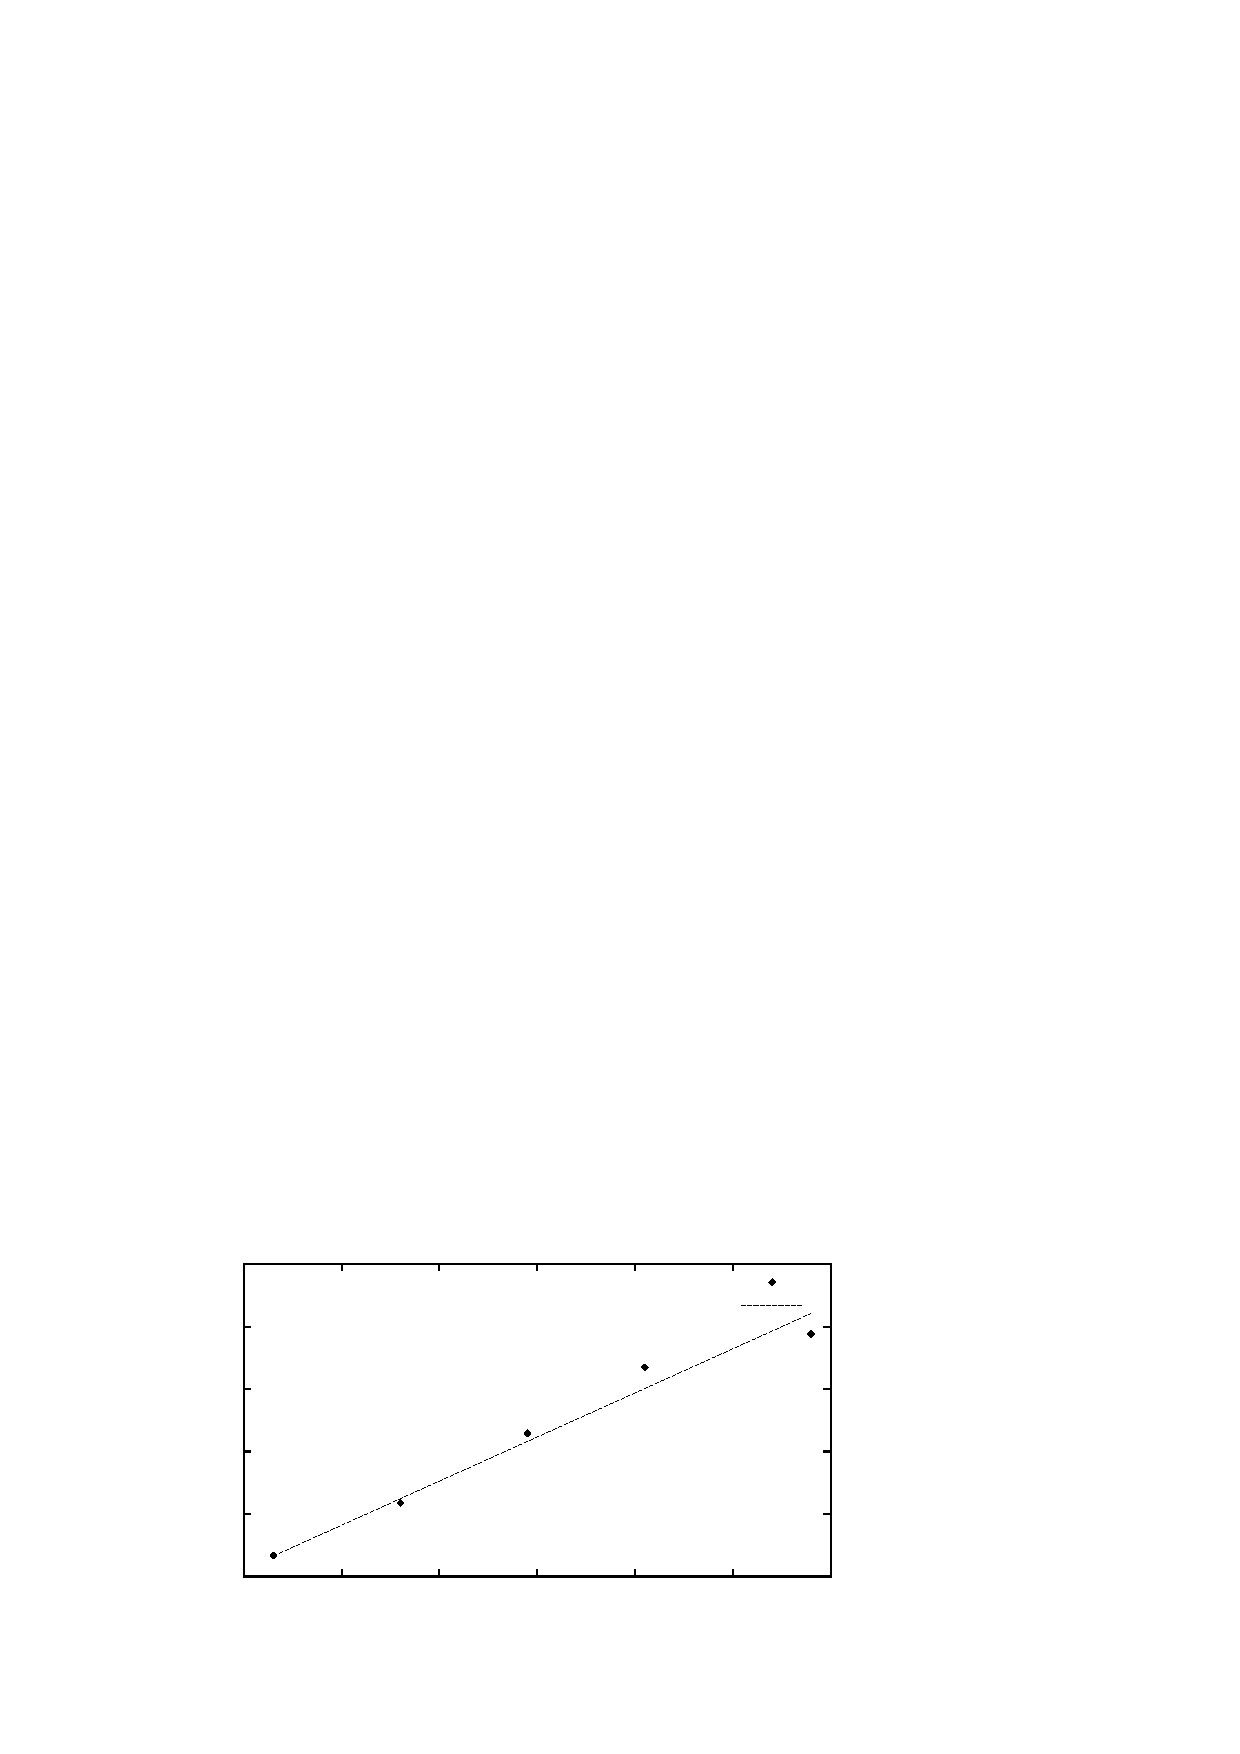
\includegraphics{antenne-01-2}}%
    \gplfronttext
  \end{picture}%
\endgroup

			\caption{\centering gemessene angepasste reziproke Frequenz $1/f$ in Abhängigkeit der Gesamtlänge $L$ einer $\lambda/2$-Antenne unter Verwendung der Schaltung aus Abbildung \ref{schaltung_antennen_1}}
			\label{diagramm_antenne_2}
		\end{figure}

		Der erwartete reziproke Zusammenhang zwischen der Länge der Antenne und der Frequenz wird anhand der Abbildung \ref{diagramm_antenne_2} deutlich.
		Hier wurde versucht eine lineare Approximation durchzuführen.
		Gewisse Abweichungen für größere Längen ergeben sich durch leichte geometrische Veränderungen der Antenne.

	% subsubsection frequenzanpassung_f_r_eine_ (end)

	\subsubsection{Empfang und Senden von Signalen} % (fold)
	\label{ssub:empfang_und_senden_von_signalen}
	
		Nach der vorangegangenen Messung war es nun möglich ein angepasstes Signal über zwei Antennen zu schicken.
		Im Folgenden betrug die Länge der zwei Antennen $88$cm. 
		Sie standen in etwa $5$m auseinander und die Sendefrequenz betrug $f^{(1)} = 164$MHz.
		Sie wurde so gewählt, um maximale Sendeleistung des Signals zu erreichen.
		Die Peak-to-Peak-Spannung wurde auf einen maximalen Wert von $U_{pp}^{(1)} = 2.28$V gesetzt.
		Mithilfe des Oszilloskops konnte dann auf der Empfängerseite eine Signal mit einer Frequenz von $f^{(2)} = 163.4$MHz und einer Peak-to-Peak-Spannung von $U^{(2)}_{pp} = 131$mV gemessen werden.
		Für das Sendeleistungsverhältnis folgt damit:
		\[
			p = \dfrac{\left(U^{(2)}_{pp}\right)^2}{\left(U^{(1)}_{pp}\right)^2} = \dfrac{131^2\text{mV}^2}{2.28^2\text{V}^2} = 3.3\cdot 10^{-3}
		\]
		Dieses Verhältnis hing im Versuchsbereich nicht vom Abstand ab.
		Wände und andere Geräte emittierten oder reflektierten so viele Wellen, dass keine Unterschiede festgestellt werden konnten.
		Für die Winkelabhängigkeit konnten folgende qualitative Messwerte aus Abbildung \ref{diagramm_antenne_3} gefunden werden.

		\begin{figure}[H]
			\center
			% GNUPLOT: LaTeX picture with Postscript
\begingroup
  \makeatletter
  \providecommand\color[2][]{%
    \GenericError{(gnuplot) \space\space\space\@spaces}{%
      Package color not loaded in conjunction with
      terminal option `colourtext'%
    }{See the gnuplot documentation for explanation.%
    }{Either use 'blacktext' in gnuplot or load the package
      color.sty in LaTeX.}%
    \renewcommand\color[2][]{}%
  }%
  \providecommand\includegraphics[2][]{%
    \GenericError{(gnuplot) \space\space\space\@spaces}{%
      Package graphicx or graphics not loaded%
    }{See the gnuplot documentation for explanation.%
    }{The gnuplot epslatex terminal needs graphicx.sty or graphics.sty.}%
    \renewcommand\includegraphics[2][]{}%
  }%
  \providecommand\rotatebox[2]{#2}%
  \@ifundefined{ifGPcolor}{%
    \newif\ifGPcolor
    \GPcolorfalse
  }{}%
  \@ifundefined{ifGPblacktext}{%
    \newif\ifGPblacktext
    \GPblacktexttrue
  }{}%
  % define a \g@addto@macro without @ in the name:
  \let\gplgaddtomacro\g@addto@macro
  % define empty templates for all commands taking text:
  \gdef\gplbacktext{}%
  \gdef\gplfronttext{}%
  \makeatother
  \ifGPblacktext
    % no textcolor at all
    \def\colorrgb#1{}%
    \def\colorgray#1{}%
  \else
    % gray or color?
    \ifGPcolor
      \def\colorrgb#1{\color[rgb]{#1}}%
      \def\colorgray#1{\color[gray]{#1}}%
      \expandafter\def\csname LTw\endcsname{\color{white}}%
      \expandafter\def\csname LTb\endcsname{\color{black}}%
      \expandafter\def\csname LTa\endcsname{\color{black}}%
      \expandafter\def\csname LT0\endcsname{\color[rgb]{1,0,0}}%
      \expandafter\def\csname LT1\endcsname{\color[rgb]{0,1,0}}%
      \expandafter\def\csname LT2\endcsname{\color[rgb]{0,0,1}}%
      \expandafter\def\csname LT3\endcsname{\color[rgb]{1,0,1}}%
      \expandafter\def\csname LT4\endcsname{\color[rgb]{0,1,1}}%
      \expandafter\def\csname LT5\endcsname{\color[rgb]{1,1,0}}%
      \expandafter\def\csname LT6\endcsname{\color[rgb]{0,0,0}}%
      \expandafter\def\csname LT7\endcsname{\color[rgb]{1,0.3,0}}%
      \expandafter\def\csname LT8\endcsname{\color[rgb]{0.5,0.5,0.5}}%
    \else
      % gray
      \def\colorrgb#1{\color{black}}%
      \def\colorgray#1{\color[gray]{#1}}%
      \expandafter\def\csname LTw\endcsname{\color{white}}%
      \expandafter\def\csname LTb\endcsname{\color{black}}%
      \expandafter\def\csname LTa\endcsname{\color{black}}%
      \expandafter\def\csname LT0\endcsname{\color{black}}%
      \expandafter\def\csname LT1\endcsname{\color{black}}%
      \expandafter\def\csname LT2\endcsname{\color{black}}%
      \expandafter\def\csname LT3\endcsname{\color{black}}%
      \expandafter\def\csname LT4\endcsname{\color{black}}%
      \expandafter\def\csname LT5\endcsname{\color{black}}%
      \expandafter\def\csname LT6\endcsname{\color{black}}%
      \expandafter\def\csname LT7\endcsname{\color{black}}%
      \expandafter\def\csname LT8\endcsname{\color{black}}%
    \fi
  \fi
  \setlength{\unitlength}{0.0500bp}%
  \begin{picture}(7370.00,3968.00)%
    \gplgaddtomacro\gplbacktext{%
      \csname LTb\endcsname%
      \put(1210,704){\makebox(0,0)[r]{\strut{} 0}}%
      \put(1210,1304){\makebox(0,0)[r]{\strut{} 5000}}%
      \put(1210,1904){\makebox(0,0)[r]{\strut{} 10000}}%
      \put(1210,2503){\makebox(0,0)[r]{\strut{} 15000}}%
      \put(1210,3103){\makebox(0,0)[r]{\strut{} 20000}}%
      \put(1210,3703){\makebox(0,0)[r]{\strut{} 25000}}%
      \put(1342,484){\makebox(0,0){\strut{} 0}}%
      \put(1968,484){\makebox(0,0){\strut{} 20}}%
      \put(2593,484){\makebox(0,0){\strut{} 40}}%
      \put(3219,484){\makebox(0,0){\strut{} 60}}%
      \put(3845,484){\makebox(0,0){\strut{} 80}}%
      \put(4470,484){\makebox(0,0){\strut{} 100}}%
      \put(5096,484){\makebox(0,0){\strut{} 120}}%
      \put(5722,484){\makebox(0,0){\strut{} 140}}%
      \put(6347,484){\makebox(0,0){\strut{} 160}}%
      \put(6973,484){\makebox(0,0){\strut{} 180}}%
      \put(176,2203){\rotatebox{-270}{\makebox(0,0){\strut{}$U^2_{pp}$ \ [mV$^2$]}}}%
      \put(4157,154){\makebox(0,0){\strut{}$\varphi$ \ [$^\circ$]}}%
    }%
    \gplgaddtomacro\gplfronttext{%
      \csname LTb\endcsname%
      \put(5986,3530){\makebox(0,0)[r]{\strut{}Messwerte}}%
      \csname LTb\endcsname%
      \put(5986,3310){\makebox(0,0)[r]{\strut{}Approximation: $f(\varphi) = a\cos^2(\varphi)$}}%
    }%
    \gplbacktext
    \put(0,0){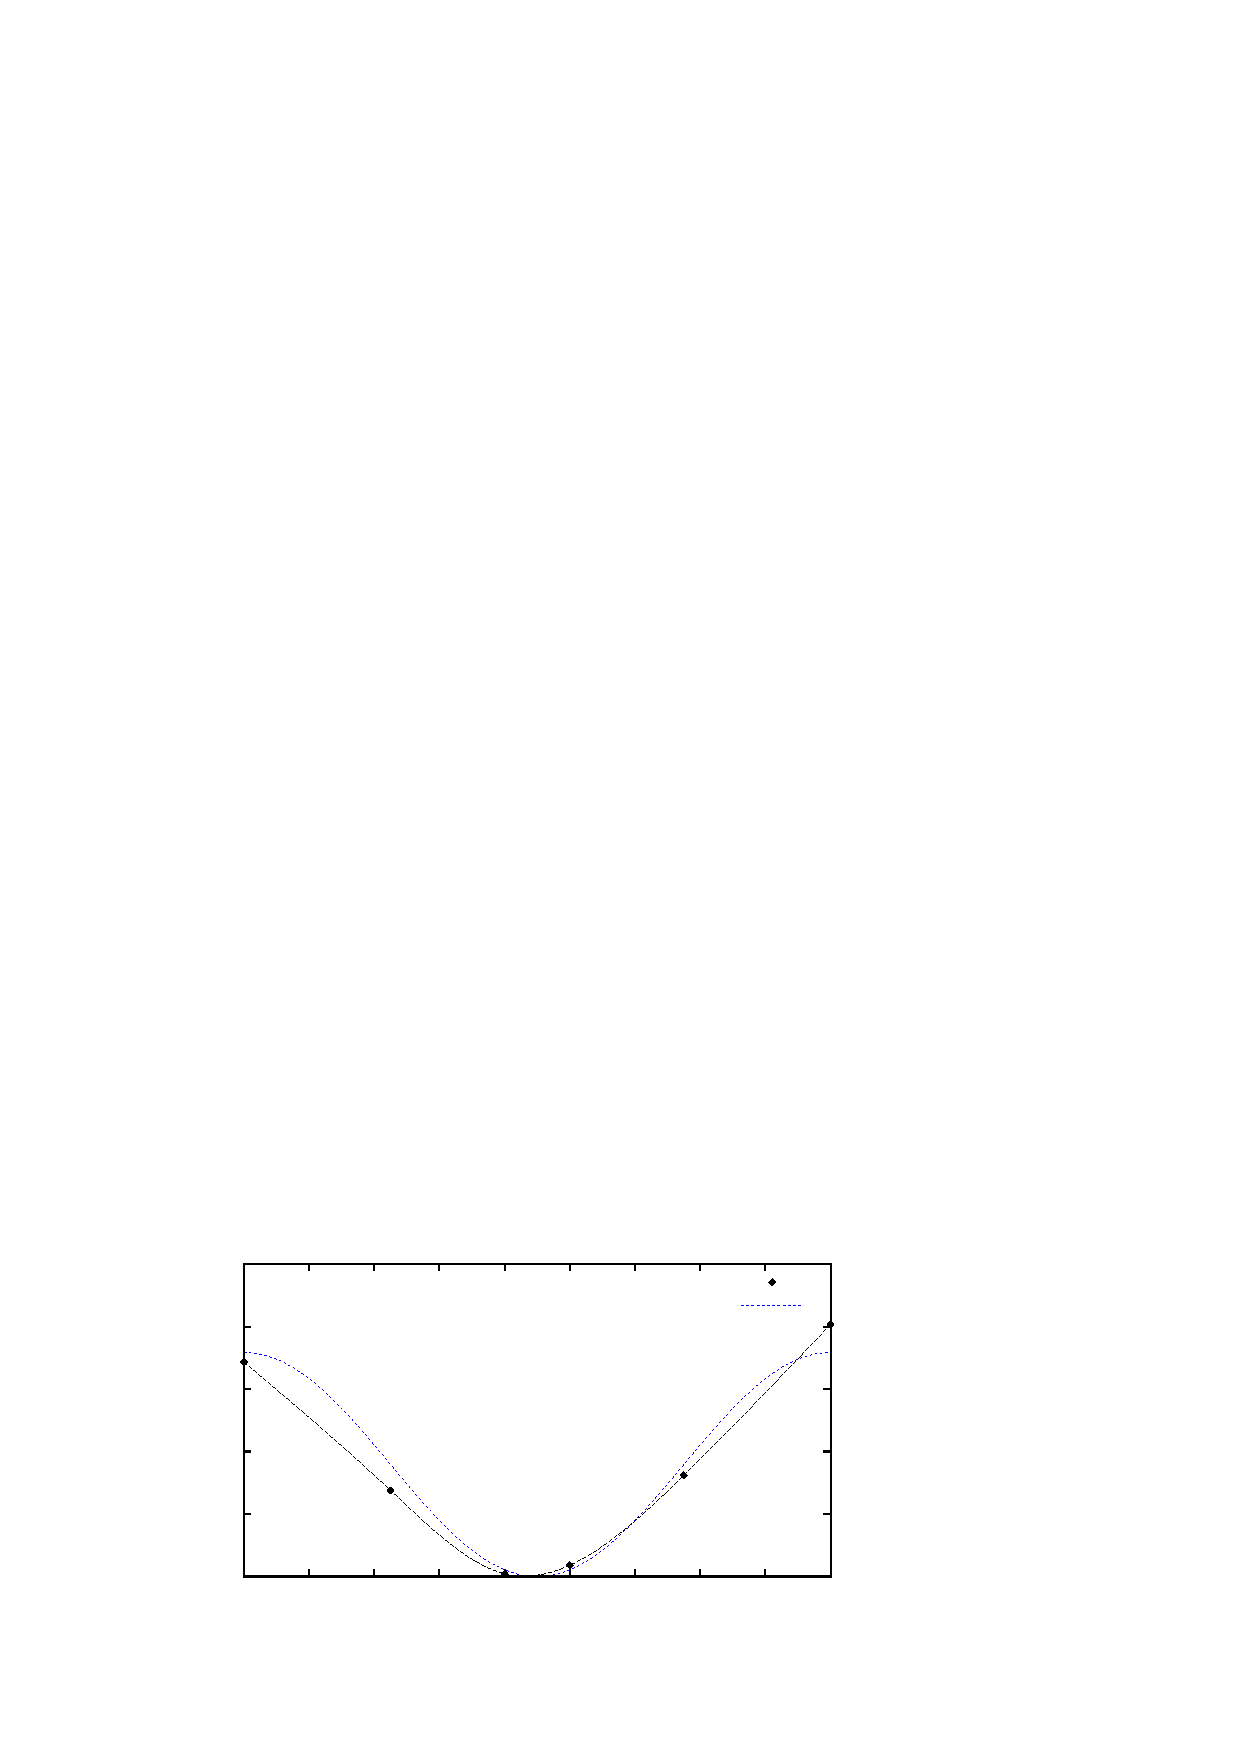
\includegraphics{antenne-02}}%
    \gplfronttext
  \end{picture}%
\endgroup

			\caption{\centering qualitative Abhängigkeit des Quadrates der Empfangsspannung $U^2_{pp}$ von dem eingestrahlten Winkel $\varphi$ unter Verwendung der Schaltung aus Abbildung \ref{schaltung_antennen_1}}
			\label{diagramm_antenne_3}
		\end{figure}

		Wie bereits erwähnt waren nur diverse qualitative Messungen möglich, da viele Wellen im Raum durch Wände und Ähnliches die Winkelabhängigkeit stark verfälschten.
		Die eingezeichnete Approximation beschreibt gerade eine typische Intensitätsverteilung im Bezug auf den Winkel.

	% subsubsection empfang_und_senden_von_signalen (end)



	\subsubsection{Signalübertragung von Musik}

	Durch Zusammennahme aller bisherigen Erkenntnisse über Modulation, Signalübertragung mittels angepasster Koaxialkabel, Möglichkeiten der additiven Amplitudenmodulation und Demodulation und optimales Abstrahlen und Empfangen von elektromagnetischen Wellen über Halbwellendipolantennen ist es nun möglich ein beliebiges niederfrequentes Signal wie beispielsweise Musik zu übertragen.
	Das Signal entstammte den analogen Klinkenanschluss eines Handys, wurde mit der unter 3.2 erklärten Schaltung und einer optimalen Trägerfrequenz von 164 MHz additiv moduliert und anschließend über die $\lambda /2$-Antenne abgestrahlt.
	Musiksignal und moduliertes Ausgangssignal wurden währenddessen über verschiedene Oszilloskope dargestellt und konnten über den gesamten Versuch beobachtet werden.
	Anschließend strahlte die unter 4.3.1 untersuchte Halbwellendipolantenne das Signal aus und eine baugleiche Antenne nahm es $5$m entfernt auf.
	Die bekannte Demodulatorschaltung gab nun wieder das niederfrequente Musiksignal aus, das ein Lautsprecher abspielte.
	Auch hier wurden empfangene und demodulierte Spannung an Oszilloskopen zeitgleich während der Übertragung untersucht. 
	Das empfangene Signal wurde auch noch einmal mit Hilfe des Spektrumanalysators im Frequenzraum dargestellt.
	Zu sehen war hier natürlich der stark ausgeprägte Peak der Trägerfrequenz von $164$ MHz sowie die Seitenbänder der Musik, die sich jedoch so stark und schnell änderten, dass daraus keine Information gewonnen werden konnte.
	Als jedoch anstelle der Musik nur ein einziger hoher Pfeifton abgespielt wurde, konnte man für den Moment eindeutig die beiden Seitenpeaks im Spektrum erkennen.
	Allgemein war das zu hörende Signal zwar immer wieder etwas durch Rauschen verzerrt und änderte Lautstärke und Qualität über die Zeit, wie auch wenn wir unsere Position im Raum veränderte, dennoch war die Musik meist klar zu erkennen und die Übertragung für den relativ einfachen Aufbau erstaunlich gut.
	Das Rauschen und die Veränderungen sind auf unregelmäßige Schwankungen der Intensität der Radiowellen in und um die Empfangsantenne zurückzuführen.
	Diese wiederum entstehen durch Beugung, Reflexion und Absorption der freien Radiowellen an Gegenständen (inklusive uns) im Raum.
	Interessanter Weise war auch von Zeit zu Zeit ein sehr regelmäßiges Schlagen, das nicht von der Musik stammte zu hören.
	Eine mögliche Quelle könnten die im Sekundentakt abgegebenen kurzen Impulse des Lasers eine Etage oberhalb sein.
	Diese sind im Spektrum so breit, dass sie auch Anteile in der von uns verwendeten Trägerfrequenz aufweisen.

	Gespielt wurde unter anderem \textit{Going to Hell} von \textit{The Pretty Reckless}.




% subsection elektromagnetische_wellen_im_freien_raum (end)